\section{Diseño y Construcción de la Computadora de Vuelo}

% Acá se da una introducción breve de esta sección, es decir, hay que explicar qué es lo que se va a mencionar acá. Se pone en contexto.

% En esta sección se describe lo que tiene la placa, es decir:
% - Cuáles son las funcionalidades que tiene la placa.
% - Arquitectura general de la placa (algo tipo diagrama en bloques).
% - Criterios tenidos en cuenta para la selección de los componentes (AEC-Q100 y pedidos del laboratorio).
% - Circuitos que implementan cada funcionalidad: selección de componentes, interfaz de comunicación con el micro y circuito diseñado.
% - Circuito completo y PCB <- Acá mencionar el motivo por el que se hizo el PCB de 4 layers y el motivo por el que todos los componentes van de un solo lado.

Como se mencionó en la sección \ref{sec:Introduccion}, la computadora de vuelo es el elemento central de un vehículo aéreo no tripulado. Su tarea principal y la más importante es la de ejecutar los algoritmos de guiado, navegación y control para mantener estable al vehículo y guiarlo en su trayectoria.

En esta sección se presentan los criterios tenidos en cuenta para el diseño y la construcción de la computadora de vuelo. Se presentan las distintas funcionalidades y el análisis de la selección de distintos componentes como sensores y circuitos integrados. Finalmente, se describe el circuito implementado y el diseño del PCB.

%\subsection{Requerimientos y Diseño General}

%\subsubsection{Implementación de Técnicas de Redundancias}

%Uso de un bus de comunicaciones TDMA, utilizado para intercambiar información y realizar algoritmos de votación. Debe poder usarse para implementar una sincronización entre nodos, en caso de que sea necesario.



%Algunos trabajos tienen salidas de control directa sobre los acutadores, la computadora de vuelo debe permitir esto.\\

%La computadora de vuelo requiere interfaces de comunicación con sensores.

%\textbf{{\color{red} COMPLETAR}}

%\subsubsection{Funcionalidades Generales}

%\textbf{{\color{red} COMPLETAR}}

\subsection{Funcionalidades de la Computadora de Vuelo}

%El Laboratorio de Automática y Robótica de la FIUBA (LAR) cuenta con plataformas de computadoras de vuelo desarrolladas en el mismo laboratorio, que se utilizan con distintos fines de investigación. Estas computadoras de vuelo han ido incorporando distintas mejoras a lo largo de los años, y se han ido actualizando con nuevos componentes como sensores o microcontroladores. La primera de las versiones cuenta con un microcontrolador ARM Cortex M3, mientras que la última de estas cuenta un ARM Cortex M7 y sensores con mejor rendimiento \cite{garberoglio2019diseno}.

%\begin{figure}[H]
%    \centering
%    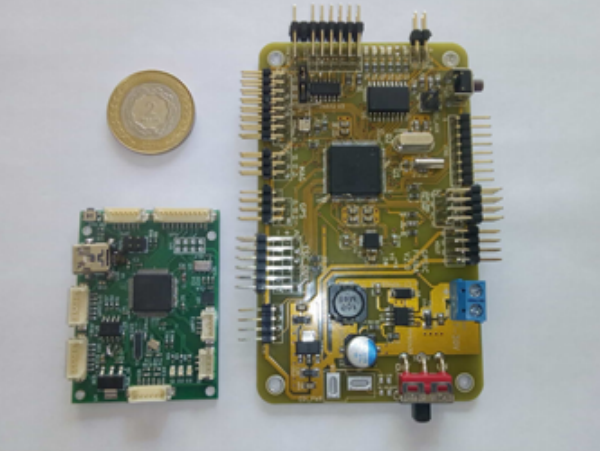
\includegraphics[width=0.5\textwidth]{choriboards_anteriores.png}
%    \caption{}    
%\end{figure}

%Hablar un poco de los sensores y componentes que tenían las computadoras anteriores y cómo fueron evolucionando.

%%%%%%%%%%%%%%%%%%%%%%%%%%%%%%%%%%%%%%%
%Todas las computadoras cuentan con un sistema de navegación inercial INS. Explicar brevemente qué es y por qué es importante.

% Tesis de Claudio:
%Los sensores inerciales son un tipo de sensores que permiten medir fuerzas específicas y velocidades de giro, mediante el uso de acelerómetros y giróscopos, generalmente ordenados en grupos de tres para medir dichos valores sobre cada eje de la terna. Este tipo de sensores permiten obtener datos a altas frecuencias, y se verá que cumplen un papel vital en la determinación de los ángulos de navegación.
%
%Dentro de los instrumentos de medición, pueden identificarse dos grupos. Por un lado, están los sensores cuyos datos son de gran importancia para la estabilidad del UAV, que son los que proveen las mediciones de los acelerómetros y giróscopos. Como ya fue mencionado, éste tipo de datos necesitan una alta frecuencia de actualización, y la demora en adquirir los datos debe ser la mínima posible.

% Tesis de Tournour
%Uno de los sistemas de navegación utilizados son los sistemas inerciales (INS por sus siglas en inglés). Estos sistemas resuelven las ecuaciones inerciales de la navegación integrando la información de los sensores. Los sensores inerciales utilizados comúnmente son los acelerómetros, para medir aceleraciones, y los giróscopos, para medir velocidades angulares. Existe una amplia variedad de sensores inerciales, pero dados los requerimientos de la aplicación en Vehículo Aéreo No Tripulado (VANT)s los que mejor se adaptan son los sensores microelectromecánicos o MEMS (del inglés Microelectromechanical MEMS Systems). Estos sensores permiten medir una amplia variedad de magnitudes, con las ventajas de su bajo costo, bajo peso, su pequeño tamaño, y su amplio ancho de banda (1kHz aprox.). En la Figura 1.2 se puede observar dos de estos sensores.

Un sistema de navegación permite realizar estimaciones de la pose del vehículo, es decir de la posición y orientación. En la figura \ref{fig:angles_drone} se muestra un UAV con una terna solidaria a este. La forma de indicar la orientación del vehículo es a través de los ángulos denominados \textit{yaw}, \textit{pitch} y \textit{roll}. Estos expresan las rotaciones entre la terna solidaria al vehículo en su posición actual, y una terna inercial, fija en el espacio.

\begin{figure}[H]
    \centering
    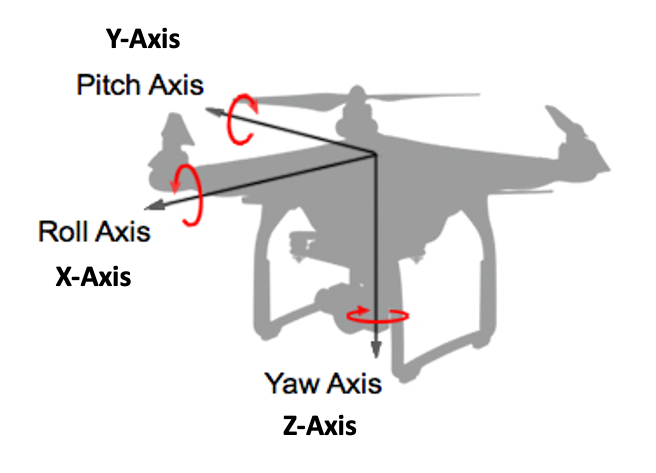
\includegraphics[width=0.5\textwidth]{angles_drone.png}
    \caption{Se utiliza una terna solidaria al vehículo para conocer su orientación en el espacio. Los ángulos \textit{yaw}, \textit{pitch} y \textit{roll} indican rotaciones respecto de una terna inercial.}
    \label{fig:angles_drone}    
\end{figure}

El principal sistema utilizado en UAVs es el sistema de navegación inercial (INS). Este consiste en realizar estimaciones de posición y orientación a partir de integrar en el tiempo mediciones de aceleración y velocidad de rotación del vehículo. Por ejemplo, podrían conocerse los ángulos de la figura \ref{fig:angles_drone} a partir de mediciones de velocidad angular. Estos sistemas no solo se utilizan en UAV sino que también en vehículos tripulados y aviones comerciales.

El hecho de integrar las mediciones de velocidad y aceleración en el tiempo, trae consigo que cualquier error de los acelerómetros y los giróscopos decante en errores de posición y de orientación que crecerán con el paso del tiempo a un ritmo acelerado. Típicamente esto se corrige utilizando otro sistema de navegación auxiliar (como por ejemplo a través de GPS) junto con un filtro de Kalman o un sistema equivalente. %En la figura \ref{fig:kalman} se muestra un diagrama en bloques que relaciona al sistema inercial con el sistema auxiliar a través del filtro de Kalman para corregir las salidas del sistema de navegación inercial.

% \begin{figure}[H]
%     \centering
%     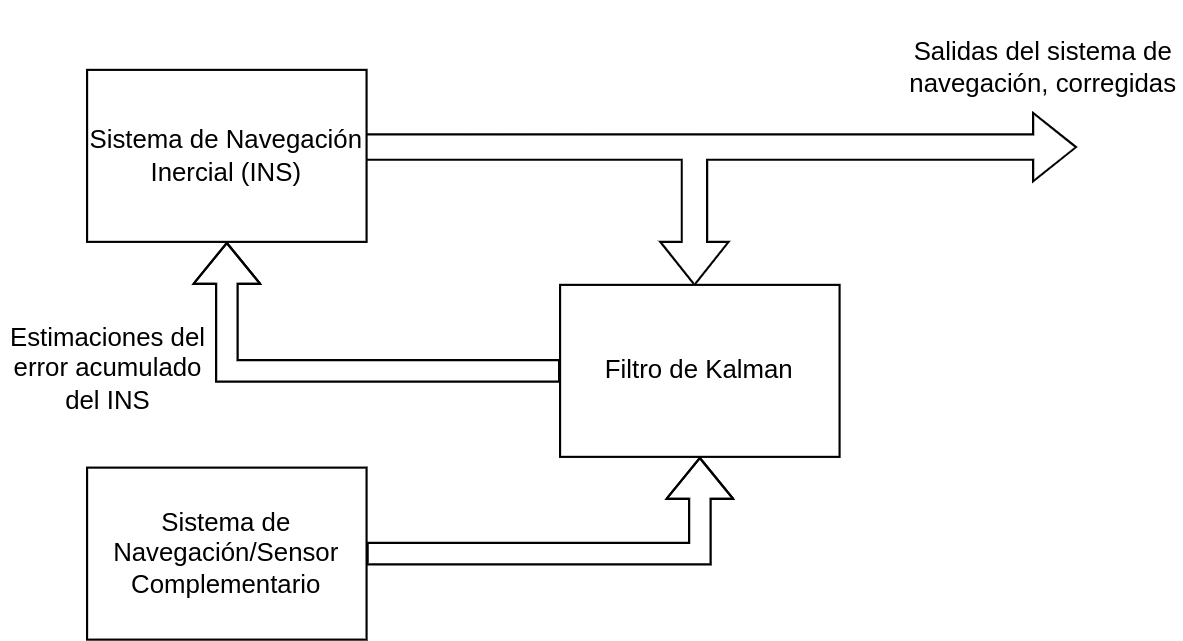
\includegraphics[width=0.8\textwidth]{kalman.png}
%     \caption{Diagrama en bloques del INS junto con un sistema de navegación auxiliar de GPS. Ambos se complementan a partir del filtro de Kalman.}
%     \label{fig:kalman}
% \end{figure}

Para obtener las mediciones de aceleración y velocidad angular en la computadora de vuelo, se utilizará una Unidad de Medición Inercial (IMU). Esta comprende acelerómetros y giróscopos triaxiales, los cuales se denominan sensores inerciales. La IMU ofrece una alta tasa de adquisición de datos, en el orden de las decenas de kHz. Esto es de gran importancia para mantener la estabilidad del vehículo, ya que utilizando acelerómetros y giróscopos es posible estimar los ángulos de \textit{pitch} y \textit{roll} del vehículo. 

%%%%%%%%%%%%%%%%%%%%%%%%%%%%%%%%%%%%%%%

% El sistema de navegación inercial requiere que se resuelvan muchas ecuaciones. Para eso se incorpora una unidad de procesamiento:
%
% Por qué se usa un microcontrolador COTS?
% - Bajo costo
% - Tamaño reducido.
% - La gran cantidad de interfaces que integran.
% - Necesidad de una respuesta con determinismo temporal.

Para realizar todos los cálculos involucrados en el INS, se utiliza una unidad de procesamiento. Todas las tareas involucradas en navegación y control de vuelo son ejecutadas de forma periódica por la computadora de vuelo. Se requiere asegurar un determinismo temporal en la ejecución de las tareas, del orden de los milisegundos o decenas de milisegundos. La unidad de procesamiento que mejor se ajusta a las necesidades de este trabajo es un microcontrolador de 32 bits, siendo el principal motivo la gran variedad que pueden encontrarse en el mercado, los cuales ofrecen una muy buena performance por un bajo costo. La gran capacidad de cómputo que ofrecen permite que este además puede realizar otras tareas más, como encargarse de la tolerancia a fallas, el almacenamiento de datos y otras tareas relacionadas a la misión del vehículo.

Otro factor importante es el gran nivel de integración que ofrecen, incorporando gran variedad y cantidad de periféricos e interfaces de comunicación. Esto favorece la posibilidad de obtener un diseño para la computadora de vuelo de dimensiones pequeñas.

Algunas de las funcionalidades secundarias que se implementan son el control de LEDs indicadores de propósito general y la capacidad de almacenamiento de datos en una memoria externa, tanto de sensores como de datos pertinentes a la misión del vehículo. De manera de ampliar las capacidades de uso, se incorpora una gran variedad de conectores que facilitan la comunicación con dispositivos y sensores externos. Esto le da una gran versatilidad, permitiendo su utilización en distintas aplicaciones de UAVs y vehículos no tripulados en general.

%Se aprovechan las distintas interfaces que ofrecen estos componentes para 

%Para realizar los cálculos se integra una unidad de procesamiento. Teniendo en cuenta versiones anteriores de la computadora de vuelo, se utiliza un microcontrolador ARM. Además de la retrocompatibilidad con versiones anteriores. Esta también será la unidad central de la placa, encargándose de las tareas de tolerancia a fallas, almacenamiento de datos y otras tareas relacionadas a la misión del vehículo.

%Es un sistema de tiempo real, se requiere determinismo en el cálculo.

%Necesidad de tener un tamaño reducido.

%%%%%%%%%%%%%%%%%%%%%%%%%%%%%%%%%%%%%%%

%no está pensada para usarse en un único tipo de vehículo, sino que puede utilizarse en vehículos con distintas arquitecturas. Esto implica la necesidad de interfaces varias para conectar módulos y sensores.

%%%%%%%%%%%%%%%%%%%%%%%%%%%%%%%%%%%%%%%

%La computadora de vuelo debe tener cierta versatilidad para implementar distintas arquitecturas redundantes para la implementación de la tolerancia a fallas.

%%%%%%%%%%%%%%%%%%%%%%%%%%%%%%%%%%%%%%%

%Otras de las funcionalidades son el control de LEDs indicadores de propósito general y la capacidad de almacenamiento de datos, tanto de sensores como de datos pertinentes a la misión del vehículo. A lo largo de esta sección se irán mencionando otras funcionalidades secundarias.

% El modelo de este componente se ha ido actualizando con las distintas versiones. Con el pasar de los años, los modelos de las primeras versiones se han ido disconinuando, dando paso a nuevos sensores que ofrecen mejores prestaciones, como por ejemplo en cuanto a ruido, offset, sensibilidad, entre otros.

% Los componentes comunes son la IMU, el uso de un microcontrolador cortex MX, salidas PWM para control de motores, tienen muchos puertos auxiliares para conectar varias cosas externas. 

% La placa desarrollada en este trabajo es una nueva versión de la computadora de vuelo. Se busca tal cosa...

%Mencionar que ya existían otras placas previas del LAR y que ahora se está haciendo una versión nueva.

%La computadora debe ser versátil, en el sentido de que no está pensada para usarse en un único tipo de vehículo, sino que puede utilizarse en vehículos con distintas arquitecturas.

%Actualización de los componentes y sensores para mejorar el rendimiento y reemplazar dispositivos obsoletos y/o discontinuados.

%Retrocompatibilidad con módulos de firmware desarrollados para la versión anterior. También retrocompatibilidad en los conectores, de manera de conectar módulos que se utilizaron en la versión anterior.

%Electrical transmission of signals and commands is a key element in a FBW system. Modern systems use a serial digital data transmission system with time division multiplexing. The signals can then be transmitted along a network or highway comprising two wires only, as only one set of data is being transmitted at any particular time. Figure 4.2 shows how a digital flight control system is interconnected using a digital data bus.

% Entrada de programación
% Debugger
% Botón reset
% IMU (SPI)
% Barómetro Integrado (I2C)
% Magnetómetro Externo (I2C)
% GPS externo (UART)
% Salidas PWM para motores + servos para otra cosa
% DSM para Spektrum
% PPM para radios en general
% Conector fuente externa tipo pixhawk
% microSD
% LEDs Integrados para indicadores
% UARTs adicionales para conectar cosas externas
% I2C adicional
% SPI adicionales
% salidas de 5V y 3V3
% switches para distintas funcionalidades

%%%%%%%%%%%%%%%%%%%%%%%%%%%%%%%%%%%%%%%

\subsection{Criterios Generales Para la Selección de Componentes}

% Acá no se dan justificaciones de algún circuito en particular, sino que se dan justificaciones que aplican a todos los bloques. Por ejemplo, el tema del AEC-Q100 y los pedidos del laboratorio, como los pines dupont, etc.

Para el diseño y construcción de la computadora de vuelo, se tuvieron en cuenta algunos criterios comunes a todos los componentes. Estos se mencionan a continuación.

% de cada circuito, se tuvieron en cuenta distintas necesidades particulares para cada uno de ellos. A su vez, hay ciertos criterios y que son comunes a todos los circuitos. Estos se mencionan a continuación.

\subsubsection{Uso de Componentes de Grado Automotriz}

Un sistema de alta confiabilidad trae consigo un costo mayor en su desarrollo y fabricación, respecto de un sistema donde este aspecto no es tan importante. Esto es principalmente debido a la necesidad de utilizar componentes de alta calidad y confiabilidad. Para el desarrollo de este trabajo, se cuenta con un presupuesto limitado, por lo que no puede accederse a componentes con estas características.

En la búsqueda de componentes y distintas alternativas, se encontró que existen algunos que cuentan con una calificación denominada AEC-Q100. Esta calificación creada por el \textit{Automotive Electronics Council} (AEC) define una serie de requerimientos que debe cumplir un componente para garantizar que este se encuentra apto para uso en electrónica automotriz. 
%Teniendo en cuenta que en los últimos años ha crecido mucho la cantidad de equipos de electrónica en estos vehículos, un fracaso en cualquiera de ellos puede afectar el funcionamiento del automóvil.
Los componentes dentro del vehículo se ven sometidos a distintas condiciones de temperatura, humedad, etc., por lo que para considerarse aptos, estos deben garantizar un correcto funcionamiento bajo distintas condiciones. Los requierimientos definidos por el AEC en la especificación AEC-Q100: \textit{Failure Mechanism Based Stress Test Qualification for Integrated Circuits In Automotive Applications} definen una serie de pruebas de estrés de componentes para demostrar la confiabilidad de los mismos.

Teniendo en cuenta que esta calificación otorga un grado de confiabilidad superior, además del hecho de que estos no representan una gran diferencia económica respecto de aquellos de uso comercial, en aquellos casos en los que fue posible se optó por la selección de componentes con esta calificación.


%Sin embargo, en la búsqueda entre una mayor confiabilidad y un costo de fabricación no tan elevado, se buscaron componentes que presenten un grado de confiabilidad superior al 


%Esto se debe a las características de los componentes y de la electrónica, los cuales deben ser 


%Con el objetivo de mejorar la confiabilidad de la computadora de vuelo, se 


%Durante la selección de componentes para la placa, y en aquellos en los que fue posible, se optó por el uso de componentes de grado automotriz, con calificación AEC-Q100. 





%Un componente de grado automotriz está diseñado y fabricado teniendo en cuenta que este será utilizado en electrónica   

%Una de las premisas de cualquier trabajo de desarrollo de electrónica, consiste en que este sea de un bajo costo. Gracias al avance de la tecnología, en los últimos años se han ido abaratando los costos de fabricación de chips y componentes electrónicos. Haciendo una búsqueda rápida en sitios web de distintos proveedores de componentes puede encontrarse que existe una gran variedad de estos, como sensores y microcontroladores, a precios razonables.

%En el caso particular de sistemas críticos, el aspecto más importante y fundamental es el de la confiabilidad. Generalmente este requerimiento impacta en el costo del desarrollo, ya que la confiabilidad suele traer consigo altos costos de fabricación. Por ejemplo, % AGREGAR EJEMPLOS DE COMPONENTES USADOS EN AVIONES.

% ENTONCES, SE QUIERE HACER ALGO SAFETY-CRITICAL PERO DE BAJO COSTE. ==> MENCIONAR LA OFERTA DE COMPONENTES AUTOMOTRIZ Y HABLAR DE AEC-Q100

%The AEC-Q100 standard is a set of rigorous requirements and tests that electronic components must pass to ensure their suitability for use in automotive applications. Since the automotive industry requires electronic components that can perform reliably in harsh environments and under demanding conditions, the AEC-Q100 is an industry standard specification that helps to ensure the quality and reliability of electronic components used in automotive applications.

%Electrical components for vehicles are subjected to plenty of stress and operate under dynamic conditions. To this end, AECs qualification, which primarily applies to packaged ICs, is centered on both reliability and longevity. Stress testing in the design phase, in turn, births stronger, more-predictable automotive systems. 

%As a result, this accumulation of electronic devices, subsystems, and functions has fostered a new urgency and intensity to the eternal problem of end-product reliability and longevity. Vehicle owners wont tolerate breakdowns in functions or features, while manufacturers cant afford the cost of recalls or in-warranty repairs.

%\textbf{{\color{red} COMPLETAR}}

\subsubsection{Longevidad}

%Quizás uno de los criterios más importantes es el de la longevidad de los componentes. En un desarrollo de electrónica se seleccionan componentes de muchos fabricantes. 

Para el desarrollo de la placa se buscaron componentes para los cuales el fabricante garantice la longevidad antes de entrar en fin de vida útil. En el eventual caso de que un componente deje de ser fabricado, a futuro esto impactará en el diseño, ya que será necesario buscar un reemplazo del mismo, para poder fabricar nuevas unidades. Algunas veces esto es directo, ya que algunos fabricantes ofrecen compatibilidad en los terminales de componentes de mismas funcionalidades. Sin embargo en otros casos, esto puede traer consecuencias como la necesidad de modificar el diseño original, además de volver a realizar pruebas del circuito, utilizando el nuevo componente. En el caso de que se trate de un sensor, incluso puede requerir la modificación del driver utilizado para interactuar con este.

Para la computadora de vuelo de este trabajo, se buscó tener una longevidad de 10 años.

%\textbf{{\color{red} COMPLETAR}}

\subsubsection{Requerimientos de Conectores}

La computadora de vuelo cuenta con una serie de conectores que permiten el agregado de dispositivos externos a la placa. Por una necesidad de compatibilidad con distintos sensores y módulos que son comúnmente utilizados con otras computadoras de vuelo, se utilizaron 2 tipos de conectores distintos. Estos se muestran en la figura \ref{fig:conectores_dupon_df_13}.

\begin{figure}[H]
    \centering
    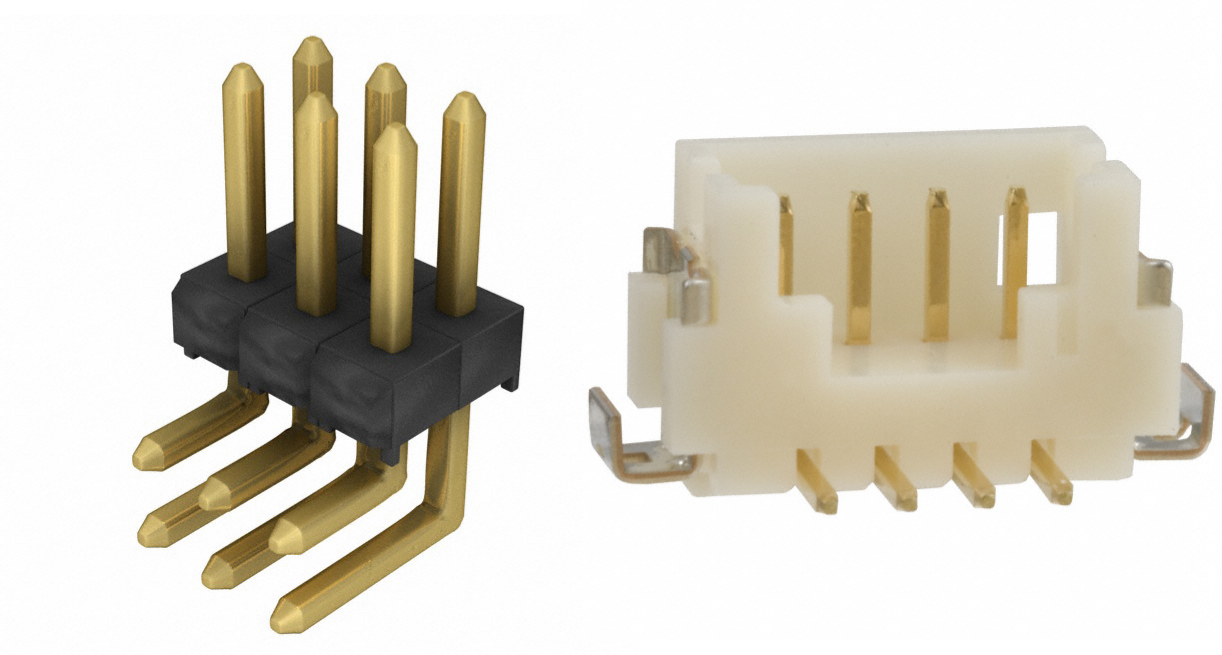
\includegraphics[width=0.5\textwidth]{img/conectores_dupon_df_13.png}
    \caption{Formato de los conectores utilizados para sensores y módulos externos en la placa. A la izquierda se muestra un conector con formato tira de pines de 0.1” a 90° y a la derecha se muestra un conector de 4 terminales, correspondiente a la serie DF-13 del fabricante Hirose.}
    \label{fig:conectores_dupon_df_13}
\end{figure}

\subsection{Circuitos y Componentes Seleccionados}

A continuación se describe cada una de las partes del circuito que conforman a la computadora de vuelo. Además de los criterios generales ya mencionados, se mencionan los criterios particulares tenidos en cuenta para cada parte del circuito.

%\subsection{Circuitos Implementados}
\subsubsection{Microcontrolador}

% Acá sí, va una subsubsection por cada bloque, por ejemplo microcontrolador, IMU, Barómetro, bus CAN, Tarjeta Micro SD, Interfaz USB, etc.

%\subsubsection{Microcontrolador}
%\subsubsection{Selección del Componente}

En la versión anterior de la computadora de vuelo, se utilizó un microcontrolador del fabricante ST, en particular el modelo STM32F722. Este cuenta con un procesador ARM Cortex-M7, que puede utilizarse con una frecuencia máxima de 216 MHz. Cuenta con unidad de punto flotante integrada, además de una memoria flash con 512 KB y una memoria RAM de 256 KB.

A todas las funcionalidades de la computadora de vuelo, en este trabajo se le suman los aspectos relacionados a la tolerancia a fallas. A su vez, se tiene la necesidad de integrar otras funcionalidades que llevan consigo una gran carga computacional. Estas pueden ser propias de la aplicación del vehículo o bien relacionadas a mejorar los algoritmos de navegación y control. Para la versión desarrollada en este trabajo, se buscó actualizar el microcontrolador a uno con mayor rendimiento, sin perder de vista la necesidad de mantener un costo reducido.

Se buscó un microcontrolador del mismo fabricante ST, de manera de tener retrocompatibilidad en el desarrollo del firmware con la versión anterior. De esta forma, muchos de los módulos de firmware que ya se encuentran desarrollados pueden reutilizarse en esta nueva versión. Con estos requerimientos, se analizaron las distintas ofertas del mercado. Además de los aspectos mencionados, se tuvieron en cuenta los periféricos presentes en cada modelo, junto con las capacidades de memorias flash y RAM. Se buscó mantener las capacidades de estas memorias en valores similares a las de la versión anterior de la computadora de vuelo.

Como primera opción surgió la posibilidad de seleccionar alguno de los microcontroladores de la serie STM32H7. Estos cuentan con procesadores ARM Cotex-M7, y pueden llegar a velocidades entre 400 MHz y 550 MHz \cite{AN5293}, es decir, pueden llegar hasta a duplicar la performance respecto de la versión anterior de la computadora de vuelo. En la tabla \ref{tab:comparacion_MCUs} se muestran distintos modelos que fueron considerados durante la selección del microcontrolador.

\begin{table}[H]
    \centering
    \begin{tabular}{|c||c|c|c|c|c|c|}
        \hline
                        & STM32F722 & STM32H723ZG & STM32H743 & STM32H753 & STM32H735ZG \\
        \hline
        Flash [kB] & 512 & 1024 & \cellcolor{green!25}1024/2048 & \cellcolor{green!25}2048 & 1024\\
        \hline
        SRAM [kB]  & 256 & 564 & \cellcolor{green!25}1024 & \cellcolor{green!25}1024 & 564\\
        \hline
        Freq [MHz] & 216 & \cellcolor{green!25}550 & 480 & 480 & \cellcolor{green!25}550\\
        \hline
        UART & 4 & \cellcolor{green!25}6 & 4 & \cellcolor{green!25}6 & \cellcolor{green!25}6\\
        \hline
        USART & 4 & \cellcolor{green!25}5 & 4 & \cellcolor{green!25}5 & \cellcolor{green!25}5\\
        \hline
        SPI & 5 & \cellcolor{green!25}6 & \cellcolor{green!25}5/6 & \cellcolor{green!25}6 & \cellcolor{green!25}6\\
        \hline
        I2C & 3 & \cellcolor{green!25}5 & 4 & 4 & \cellcolor{green!25}5\\
        \hline
        CAN & 1 & \cellcolor{green!25}3 & 2 & \cellcolor{green!25}3 & \cellcolor{green!25}3\\
        \hline
        ADC & 3x12b, 24ch & \makecell{2x16b, 22 ch; \\ 1x12b, 12 ch} & \cellcolor{green!25}\makecell{3x16b, \\ 16/28/32ch} & \makecell{1x12b, 12ch \\ 2x16b, 18ch} & \makecell{1x12b, 12ch \\ 2x16b, 16ch}\\
        \hline
        Timers & \makecell{18: 16b x 16, \\ 32b x 2} & \cellcolor{green!25}\makecell{21: 16b x 17, \\ 32b x 4} & \makecell{14: 16b x 12, \\ 32b x 2} & \cellcolor{green!25}\makecell{21: 16b x 17, \\ 32b x 4} &\cellcolor{green!25} \makecell{21: 16b x 17, \\ 32b x 4}\\
        \hline
        SDMMC & \cellcolor{green!25}2 & \cellcolor{green!25}2 & \cellcolor{green!25}2 & \cellcolor{green!25}2 & \cellcolor{green!25}2\\
        \hline
        longevidad & \cellcolor{green!25}01/2033 & \cellcolor{green!25}01/2033 & \cellcolor{green!25}01/2033 & \cellcolor{green!25}01/2033 & \cellcolor{green!25}01/2033\\
        \hline
        AEC-Q100 & No & No & No & No & No\\
        \hline       
    \end{tabular}
    \caption{Se muestra la comparación de las distintas alternativas que fueron tenidas en cuenta para la selección del mircocontrolador. En verde se destaca el componente que tiene las mejores características para cada fila. El modelo STM32F722 corresponde al modelo utilizado en la versión anterior de la computadora de vuelo.}
    \label{tab:comparacion_MCUs}
\end{table}

Todos los microcontroladores de la serie STM32H7 presentan mejoras en cuanto a frecuencia de operación, memoria flash y RAM. Sumado a esto, la gran mayoría de estos microcontroladores se encuentran dentro del programa \textit{Longevity Commitment} \cite{longevity_ST}. El fabricante ST se compromete a mantener la producción de los componentes que se encuentren dentro de este programa durante un período determinado. Todos los microcontroladores de la tabla \ref{tab:comparacion_MCUs} tienen un periódo de fabricación de 10 años asegurado por ST, finalizando en 01/2033. Este aspecto es de especial interés teniendo en cuenta la posible necesidad futura de fabricar nuevas placas de la computadora de vuelo.

\textbf{{\color{red} COMPLETAR POR QUÉ NO SE ELEIGIÓ UNO AEC-Q100, QUE ES PORQUE NO HABÍA CORTEX M7 DE ST QUE SEA AEC-Q100}}

%\textbf{{\color{red} COMPLETAR LA JUSTIFICACIÓN DE QUE SE ELIGIÓ UN MICROCONTROLADOR DIFERENTE DEBIDO A LA CRISIS Y FALTANTE DE CHIPS}}

% Acá lo importante es decir que se quería elegir un controlador más potente que la choriboard III, algún STM32H7. Mencionar por qué STM32, que es porque ellos vienen trabajando con esos microcontroladores. Luego explicar que debido al faltante y la crisis, se tuvo que elegir otro controlador. También, mencionar que el que se eligió tiene 10 años de garantía de fabricación, lo que favorece la longevidad.

A pesar del análisis y de las comparaciones entre microcontroladores de la serie STM32H7, la selección del microcontrolador se vio limitada por la disponibilidad de componentes encontrada durante el período de desarrollo del circuito.

\textbf{{\color{red} SE PUEDE SIMPLEMENTE MENCIONAR LA CRISIS DE CHIPS COMO CAUSA DE LA FALTA DE DISPONIBILIDAD.}}

El microcontrolador seleccionado fue el STM32F746ZG. Este cuenta con un procesador ARM-Cortex M7, 1024 kB de memoria flash y 320 kB de memoria SRAM. Un aspecto relevante de este microcontrolador es que cuenta con 2 interfaces para uso de un bus denominado Controller Area Network (CAN), el cual se utilizará para establecer las comunicaciones relevantes a los algoritmos de tolerancia a fallas. La posibilidad de contar con dos de estas interfaces permite implementar un sistema donde este bus no sea un punto singular de falla.

Suamdo a las prestaciones, este micocontrolador cuenta con un encapsulado LQFP de 144 terminales, lo que permite realizar muchas conexiones con sensores y componentes a través de distintas interfaces comunes, como SPI, I2C, además de terminales GPIO comunes para interrupciones y manejo de otros módulos.

\textbf{{\color{red} SE PUEDE EXPLICAR LA SELECCIÓN DE LOS CRISTALES Y EL USO DE LOS CAPACIOTRES DE DESACOPLE, SIGUIENDO LA APP NOTE DE ST.}}

% Mencionar cómo se asignaron los distintos timers para su uso en la aplicación.


% Mencionar cómo se asignaron las interrupciones externas de gpios.

% Acá también hay que mencioanr todos los cálculos y justificaciones para la selección del cristal, tanto de 12 MHz como el de 32 kHz. Poner todo lo que tengo, esta sección tiene muchísimo para mostrar.

%\textbf{{\color{red} COMPLETAR}}

%\subsection{Otros Circuitos Implementados}

%\subsubsection{Sensor IMU}

%\subsubsection{Requerimientos del Componente}

%\textbf{{\color{red} COMPLETAR}}

% acá van todos los capacitores de desacople, etc

%\subsubsection{Cristal Externo}

%\textbf{{\color{red} COMPLETAR}}

%\subsubsection{Cristal para RTC}

%\textbf{{\color{red} COMPLETAR}}

\subsubsection{Sensor IMU}\label{sec:IMU}

La unidad de medición inercial, IMU por sus siglas en inglés, es el sensor principal utilizado por la computadora de vuelo. Este consiste en un circuito integrado que contiene una serie de sensores inerciales, en particular acelerómetros y giróscopos triaxiales. Los acelerómetros se utilizan para realizar mediciones de aceleración lineal y los giróscopos para medir velocidad angular. A partir de estas mediciones, se pueden aplicar distintos algoritmos de procesamiento para obtener una estimación de la posición y orientación del vehículo. Las mediciones de aceleración lineal y de velocidad angular que entrega la IMU son referidas a una terna solidaria al componente, como se muestra en la figura \ref{fig:IMU_ejes}.

\begin{figure}[H]
    \centering
    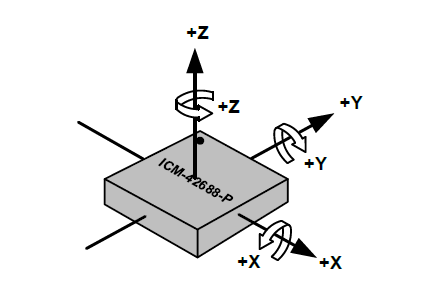
\includegraphics[width=0.4\textwidth]{img/IMU_ejes.png}
    \caption{Todas las mediciones que entrega el sensor son realtivas a una terna solidaria a este. La imagen se extrajo de \cite{ICM42688pDatasheet}.}
    \label{fig:IMU_ejes}
\end{figure}

Los acelerómetros y giróscopos de la IMU utilizada en este trabajo, se construyen utilizando la tecnología MEMS: \textit{Micro Electro-Mechanical Systems}. Esta consite en utilizar técnicas de fabricación de circuitos integrados para integrar en el silicio partes que móviles que constituyen los sistemas mecánicos de los acelerómetros y giróscopos. Este tipo de sensores tienen la ventaja de que pueden conseguirse por un bajo costo, además de tener encapsulados muy pequeños, permitiendo obtener un diseño de dimensiones reducidas. 


%En la figura \ref{fig:MEMS_acelerometro}, se muestra una imagen tomada con un microscopio electrónico de un acelerómetro MEMS. Lo que se observa en este caso, es que en el mismo silicio se integra una masa llamada \textit{proof-mass}, la cual se encuentra sujeta al sustrato a través de dos resortes.



%Esta consiste en integrar sistemas mecánicos de dimensiones microscópicas en el mismo silicio del chip, junto el resto del circuito. 



%Utilizando técnicas de fabricación de circuitos integrados, se construyen los acelerómetros y giróscopos, integrando en el silicio partes que son móviles. En la figura \ref{fig:MEMS_acelerometro}, se muestra una imagen tomada con un microscopio electrónico de un acelerómetro MEMS. Lo que se observa en este caso, es que en el mismo silicio se integra una masa llamada \textit{proof-mass}, la cual se encuentra sujeta al sustrato a través de dos resortes.

% \textbf{{\color{red} REEMPLAZAR LO QUE SIGUE POR UNA SIMPLE MENCIÓN DE SENSORES MEMS, DESDE ACÁ:}}

% Los acelerómetros y giróscopos de la IMU utilizada en este trabajo, se construyen utilizando la tecnología MEMS: \textit{Microelectromechanical Systems}. Utilizando técnicas de fabricación de circuitos integrados, se construyen los acelerómetros y giróscopos, integrando en el silicio partes que son móviles. En la figura \ref{fig:MEMS_acelerometro}, se muestra una imagen tomada con un microscopio electrónico de un acelerómetro MEMS. Lo que se observa en este caso, es que en el mismo silicio se integra una masa llamada \textit{proof-mass}, la cual se encuentra sujeta al sustrato a través de dos resortes.

% \begin{figure}[H]
%     \centering
%     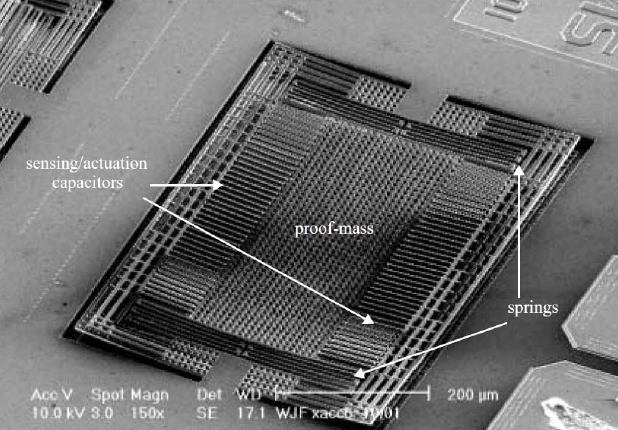
\includegraphics[width=0.6\textwidth]{img/MEMS_acelerometro.png}
%     \caption{Fotografía tomada de un acelerómetro construido con tecnología MEMS. La imagen se extrajo de \cite{zhang2010sensing}. }
%     \label{fig:MEMS_acelerometro}    
% \end{figure}

% Una aceleración sobre el componente genera que la masa del acelerómetro se mueva. Estos desplazamientos producen una variación en la capacidad existente entre el sustrato y la masa, lo que lleva a una variación de la tensión entre ambos. Esta diferencia de potencial variable es medida por un circuito dentro del chip, y que luego se utiliza para generar las mediciones de aceleración.\\

% El acelerómetro puede modelarse de manera simple, como un sistema mecánico con una masa, un resorte y un amortiguador \cite{zhang2010sensing}, como se muestra en la figura \ref{fig:acelerometro_modelo}.

% \begin{figure}[H]
%     \centering
%     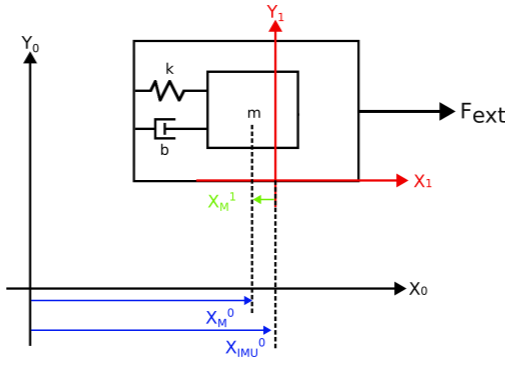
\includegraphics[width=0.5\textwidth]{img/acelerometro_modelo.png}
%     \caption{Sistema mecánico simplificado del acelerómetro.}
%     \label{fig:acelerometro_modelo}    
% \end{figure}

% La terna 0 corresponde a una terna inercial, mientras que la terna 1 es no inercial, solidaria al movimiento del acelerómetro. Cabe aclarar que tal como se mencionó, la masa se encuentra sujeta al sustrato solamente a través del resorte. El elemento amortiguador representa pérdidas de energía, causadas por rozamiento con el aire o de la propia estructura electromecánica. Se puede resolver el sistema mecánico, tomando como coordenadas generalizadas $q_1 = X_{IMU}^0$ y $q_2 = X_M^1$. Sin considerar efectos de la gravedad, se llega a la ecuación \eqref{eq:acelerometro_segundo_orden}. Este es un sistema de segundo orden, donde la entrada es la aceleración del acelerómetro y la salida es el desplazamiento de la masa respecto de la terna solidaria al acelerómetro. 

% \begin{equation}
%     \ddot{X_M^1} + \frac{b}{m} \dot{X_M^1} + \frac{k}{m} X_M^1 = -\ddot{X_{IMU}^0}
%     \label{eq:acelerometro_segundo_orden}
% \end{equation}

% Como resultado interesante, se observa que el sistema es de segundo orden, típicamente con respuesta sub-amortiguada. Algunos fabricantes de estos sensores indican en sus hojas de datos, un valor de frecuencia de resonancia. Este valor resulta de interés ya que si se excita al sensor con frecuencias cercanas a la resonancia, dejará de funcionar como dispositivo para medir la aceleración lineal. Por otro lado, a muy bajas frecuencias se puede despreciar la velocidad de la masa y luego se obtiene una relación directa entre la aceleración del acelerómetro y el desplazamiento de la masa, ecuación \eqref{eq:relacion_aceleracion_despalzamiento}.

% \begin{subequations}
% 	\begin{align}
%         \ddot{X_M^1} &\approx 0\\
%         \dot{X_M^1} &\approx 0\\
%         \frac{k}{m} X_M^1 &\approx -\ddot{X_{IMU}^0}
% 	\end{align}
%     \label{eq:relacion_aceleracion_despalzamiento}
% \end{subequations}

% El desplazamiento de la masa produce una variación de la capacidad entre esta y el sustrato. Esta capacidad es utilizada para medir una varaición de tensión \cite{zhang2010sensing}. El circuito medido puede modelarse como en la figura \ref{fig:acelerometro_sensado_capacitivo}.

% \begin{figure}[H]
%     \centering
%     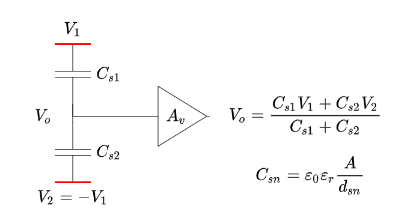
\includegraphics[width=0.5\textwidth]{img/acelerometro_sensado_capacitivo.png}
%     \caption{Circuito equivalente que mide el desplazamiento de la masa. Las tensiones $V1$ y $V2$ representan señales de tensión aplicadas por un circuito externo. El movimiento de la masa modifica la capcidad y por ende la tensión medida.}
%     \label{fig:acelerometro_sensado_capacitivo}    
% \end{figure}

% Se puede resolver este circuito y llegar a que existe una relación lineal entre la tensión $Vo$ y el desplazamiento de la masa $\Delta d$, ecuación \eqref{eq:tension_salida_acelerometro}. En \cite{zhang2010sensing} puede encontrarse la demostración completa. En la ecuación, $d_0$ representa la separación de reposo entre el sensor y el sustrato y $\Delta d$ la variación de la separación.

% \begin{equation}
%     V_{o} = \frac{\Delta d}{d_0} V_1
%     \label{eq:tension_salida_acelerometro}
% \end{equation}

% \textbf{{\color{red} HASTA ACÁ}}

%\textbf{{\color{red} COMPLETAR UN ANÁLISIS SIMILAR PARA EL GIRÓSCOPO}}

Se hizo una búsqueda de las distintas alternativas existentes para este tipo de sensores. A partir de leer las hojas de datos de distintos fabricantes, se encontró que los parámetros típicamente especificados, tanto para los acelerómetros como para los giróscopos, son los siguientes:

\begin{itemize}
    \item \textit{Full-scale range}
    \item \textit{Sensitivity}
    \item \textit{Scale factor error}
    \item \textit{Scale factor error vs temp}
    \item \textit{Offset}
    \item \textit{Offset vs temp}
    \item \textit{Offset vs time}
    \item \textit{Noise}
\end{itemize}

El primero de ellos, el \textit{Full-scale range} es el rango de medición del sensor. Para los acelerómetros se suele especificar en un rango de $\pm n \times g$, donde $n$ es algún entero y $g$ representa la aceleración de la gravedad. Para los giróscopos, se especifica como $\pm n \times dps$, donde $dps$ significa \textit{degrees-per-second}.

El parámetro \textit{Sensitivity} hace referencia a la resolución. En algunas hojas de datos este parámetro puede encontrarse con unidades de $LSB/g$ para los acelerómetros y en $LSB/dps$ para los giróscopos. Este valor puede resultar confuso de entender, ya que lo que informa es la cantidad de bits por $g$ o la cantidad de bits por $dps$. En la figura \ref{fig:ICM_42688_datasheet} se muestra una captura de la hoja de datos del sensor seleccionado, el ICM42688p. 

\begin{figure}[H]
    \centering
    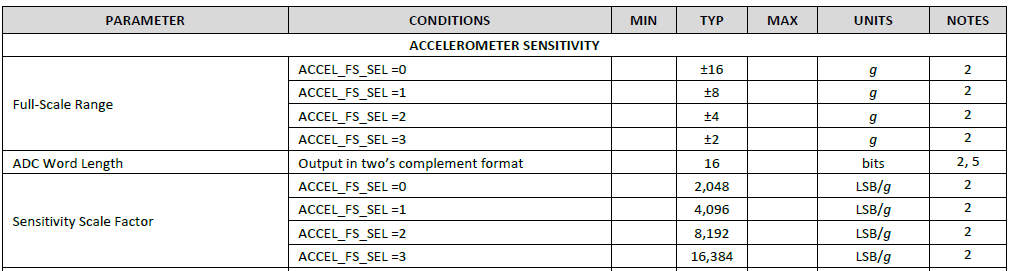
\includegraphics[width=\textwidth]{img/ICM_42688_datasheet.png}
    \caption{Extracto de la hoja de datos del sensor ICM42688p. Se muestra parte de las especificaciones para los acelerómetros.}
    \label{fig:ICM_42688_datasheet}    
\end{figure}

La imagen muestra que el sensor permite seleccionar distintos rangos de escala para las mediciones del acelerómetro. Por ejemplo, si se selecciona el rango $\pm 2g$, la hoja de datos especifica una resolución de $16384 \ LSB/g$. Una mejor forma de entender este parámetro sería si se considera la inversa, es decir, la resolución del ADC. En este caso sería de $61.04 \ 10^{-6} \ g$. Luego para un rango de $\pm 4g$ la resolución es de $8192 \ LSB/g$, es decir, $122.07 \ 10^{-6} \ g$. Este valor es el doble del anterior y tiene sentido dado que se está midiendo un rango mayor de aceleraciones utilizando la misma cantidad de bits, en este caso 16 según lo especificado en la hoja de datos.

Para entender los parámetros, \textit{scale factor error}, \textit{offset} y \textit{noise} se plantea un modelo sencillo de medición, tanto para acelerómetros como para giróscopos \cite{borodacz2022review}. Este se presenta en la ecuación \eqref{eq:medicion_vs_real}, donde $S$ es el \textit{scale factor error}, $\omega_b(t)$ es el \textit{offset} el cual es variable con el tiempo, $\eta \sim \mathcal{N}(0,\sigma^2)$, $\omega_m$ es el valor medido y $\omega$ sería la velocidad angular verdadera para el giróscopo.

\begin{equation}
    \omega_m = (1+S)\omega + \omega_b (t) + \eta
    \label{eq:medicion_vs_real}
\end{equation}

A su vez, en las hojas de datos se especifica la dependencia de estos parámetros con el tiempo y con la temperatura, como es el caso del \textit{scale factor error}.

Para tener un criterio de selección del sensor IMU, se siguió el análisis planteado en \cite{borodacz2022review}. Este paper presenta un análisis de los parámetros de los acelerómetros y grióscopos y su impacto en las estimaciones de posición en sistemas de navegación inercial (INS). En este se concluye que los parámetros más importantes para la selección del sensor son:

\begin{itemize}
    \item Estabilidad del offset de los acelerómetros (Offset vs time).
    \item Estabilidad del offset de los giróscopos (Offset vs time).
    \item Ruido de los giróscopos (Noise).
    \item Error de escala del giróscopo (Scale factor error).
\end{itemize}

Se buscaron modelos de IMUs de distintos fabricantes, para comparar características. Existe una gran cantidad de fabricantes y de componentes para seleccionar. Se buscaron componentes que sean accesibles y que no tengan un costo muy elevado. Existen IMUs de una excelente calidad, pero que tienen precios que no están al alcance (cientos o miles de dólares). Con este criterio, se realizó una comparación entre distintos modelos de sensores. En la tabla \ref{tab:comparacion_IMUs} se muestra una comparación de los distintos sensores considerados. Sumado a esto, se tuvo en consideración otro aspecto que fue mencionado anteriormente, la longevidad del componente.

\begin{table}[H]
    \centering
    \begin{tabular}{|c||c|c|c|c|c|}
        \hline
                        & ICM42688 & LSM6DSR & IIM-42652 & BMI088 & ASM330LHHX\\
        \hline
        $b_{accel}(t)$ & N/A      & N/A     & N/A       & N/A    & \cellcolor{green!25}40 $\mu$ g\\
        $b_{gyro}(t)$   & N/A      & N/A     & N/A       & \cellcolor{green!25}2°/h    & 3°/h\\
        $\eta_{gyro}$   & \cellcolor{green!25}$2.8 mdps/\sqrt{Hz}$ & $5 mdps/\sqrt{Hz}$ & $3.8 mdps/\sqrt{Hz}$ & $14 mdps/\sqrt{Hz}$ & $5 - 12 mdps/\sqrt{Hz}$\\
        $S_{gyro}$ & \cellcolor{green!25}$0.5 \%$ & $1 \%$ & \cellcolor{green!25}$0.5 \%$ & $1 \%$ & $2 \%$\\
        \hline
        longevidad & N/A & N/A & 10 años, dic. 2020 & N/A & \cellcolor{green!25}15 años, mayo 2022\\
        AEC-Q100 & No & No & No & No & \cellcolor{green!25}Sí\\
        \hline       
    \end{tabular}
    \caption{Se muestra la comparación de las distintas alternativas que fueron tenidas en cuenta para la selección del sensor. En verde se destaca el componente que tiene las mejores características para cada parámetro.}
    \label{tab:comparacion_IMUs}
\end{table}

Lo primero que llama la atención es el hecho de que muchos de los sensores no especifican todos sus parámetros. Una sola de las alternativas consideradas tiene disponible toda la información en su hoja de datos. Esto dificulta mucho la selección de un componente. A priori, se seleccionó el sensor ASM330LHHX por el hecho de ser el único que ofrece toda la información en su hoja de datos, además de ser de grado automotriz y tener una longevidad garantizada de 15 años. Teniendo en cuenta aspectos de confiabilidad, resulta esencial el hecho de conocer los parámetros del sensor.

Durante la selección del sensor hubo otro aspecto importante que se tuvo en cuenta y es el hecho de la compatibilidad con el software desarrollado por el laboratorio, para computadoras de vuelo anteriores a la de este trabajo. La versión anterior contaba con un sensor IMU ICM20602, del fabricante TDK. El laboratorio cuenta con bibliotecas de código ya desarrolladas para este sensor. Este presentó excelentes resultados, lo que sienta un antecedente importante en la selección de componentes del mismo fabricante. En la tabla \ref{tab:comparacion_IMUs_TDK} se muestra una comparación entre el sensor anterior ICM20602 y el sensor seleccionado ICM42688.

\begin{table}[H]
    \centering
    \begin{tabular}{|r||c|c|}
        \hline
         & ICM20602 & ICM42688 \\
        \hline
        Año & 2016 & 2021\\
        \hline
        \multicolumn{3}{|c|}{Giróscopos}\\
        \hline
        Full Scale Range[dps] & $\pm 250/500/1000/2000$ & $\pm 15/31/62/125/250/500/1000/2000$\\
        Scale Factor Error[\%] & $1.0$ @ 25°C & $0.5$ @ 25°C\\
        Scale factor error vs temp[\%/°C] & $0.016$ @ -40°C - 85 °C & $0.005$ @ 0°C - 70 °C\\
        Offset[dps] & $\pm 1$ & $\pm 0.5$\\
        Offset vs temp[dps/°C] & $0.01$ & $0.005$\\
        Offset vs time[°/h] & N/A & N/A\\
        Noise[$mdps/\sqrt{Hz}$] & $4$ & $2.8$\\
        \hline
        \multicolumn{3}{|c|}{Acelerómetros}\\
        \hline
        Full Scale Range[g] & $\pm 2/4/8/16$ & $\pm 2/4/8/16 $\\
        Scale Factor Error[\%] & $1.0$ @ 25°C & $0.5$ @ 25°C\\
        Scale factor error vs temp[\%/°C] & $0.012$ @ -40°C - 85 °C & $0.005$\\
        Offset[mg] & $\pm 25$ & $\pm 20$\\
        Offset vs temp[mg/°C] & X,Y: $\pm 0.5$, Z: $\pm 1$ & $\pm 0.15$\\
        Offset vs time[$\mu$g/h] & N/A & N/A\\
        Noise[$\mu g/\sqrt{Hz}$] & $100$ & X,Y: $65$, Z: $70$\\        
        \hline       
    \end{tabular}
    \caption{Se muestra la comparación del sensor ICM20602 y el sensor seleccionado ICM42688.}
    \label{tab:comparacion_IMUs_TDK}
\end{table}

Para el diseño del circuito se siguieron las recomendaciones en la hoja de datos del componente. Este sugiere incluir una serie de capacitores de desacople en los terminales de alimentación del componente. Se elige utilizar una comunicación SPI en modo esclavo, donde el maestro es el microcontrolador, ya que pueden obtenerse mayores velocidades de comunicación, respecto de otros protocolos como I2C. De esta forma se logra una alta tasa de adquisición de datos de acelerómetros y giróscopos. Como ya fue mencionado, esto resulta clave para mantener la estabilidad del vehículo. El circuito completo puede encontrarse en el \nameref{appendix:circuito_esquematico}.

Dado que el sensor IMU es un esclavo en la comunicación SPI, este solo puede comunicarse con el microcontrolador cuando este último le permita hacerlo. Para que la IMU pueda informar el momento en el que se obtuvo una nueva lectura, el sensor dispone de una salida digital la cual puede conectarse a una entrada digital del microcontroldor. Cuando el microcontrolador detecta un cambio de nivel en esta entrada, el mismo procede a solicitar el dato a través de la comunicación SPI. En la figura \ref{fig:IMU_SPI} se muestra un esquema de la conexión entre el controlador y el sensor IMU.

\begin{figure}[H]
    \centering
    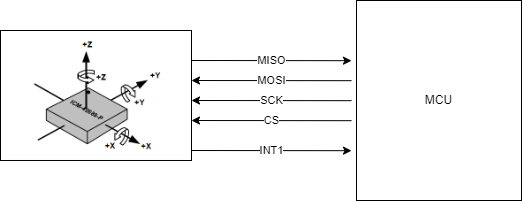
\includegraphics[width=0.8\textwidth]{img/IMU_SPI.png}
    \caption{Líneas de comunicación entre la IMU y el microcontrolador.}
    \label{fig:IMU_SPI}    
\end{figure}

\subsubsection{Barómetro}
%\subsection{Barómetro}

El barómetro se utiliza para obtener una estimación precisa de la altitud a la que está operando el UAV, a partir de mediciones de presión. Este es uno de los sensores complementarios al INS que se incorporan en la computadora de vuelo. Al igual que la IMU, el barómetro que se utiliza corresponde a un sensor de tecnología MEMS. En particular, los barómetros MEMS cuentan con un sistema capaz de medir la presión absoluta, es decir respecto al 0 de presión. Estos cuentan con una cavidad integrada dentro del chip que se encuentra (idealmente) a presión 0. %A través de un proceso llamado \textit{anodic bonding} \cite{baro_1}\cite{baro_2} se construye esta cavidad dentro del chip, la cual se encuentra sellada a una presión muy baja, en comparación con las presiones que se esperan medir utilizando el componente.
Para medir la presión, se coloca una membrana sobre la cavidad. En la figura \ref{fig:MEMS_barometro} se puede apreciar el efecto de la presión externa. 

\begin{figure}[H]
    \centering
    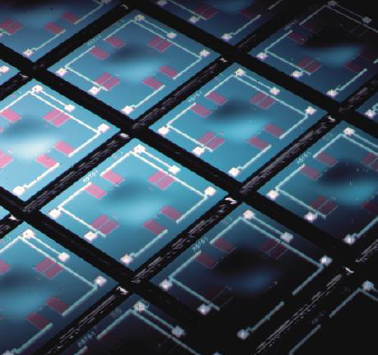
\includegraphics[width=0.4\textwidth]{img/MEMS_barometro.png}
    \caption{Sensores de presión sobre una oblea de silicio \cite{baro_1}.}
    \label{fig:MEMS_barometro}
\end{figure}

Sobre esta membrana se colocan resistores de efecto piezoresistivo en configuración puente de Wheatstone. El efecto de la presión genera compresiones y deformaciones en los resistores \cite{baro_3}, lo que se traduce en un desbalance del puente. A partir del sensado de la diferencia de potencial, se mide la presión aplicada sobre la membrana.


% En \eqref{eq:barometro_wheatstone} se despeja la relación entre la variación de tensión y la variación de la resistencia. Como se observa, la realación es proporcional.

% La deformación de la membrana genera tensión sobre estos, modificando su resistencia, de manera tal de que la presión comprime a dos de los resistores y estira a los otros dos \cite{baro_3}.


% Sobre las zonas de color violeta, se colocan resistores de efecto piezoresistivo. En consecuencia, la deformación de la membrana genera tensión sobre estos, modificando su resistencia, de manera tal de que la presión comprime a dos de los resistores y estira a los otros dos \cite{baro_3}.

% Los resistores se conectan en configuración puente de Wheatstone, de manera tal de que la presión comprime a dos de los resistores y estira a los otros dos \cite{baro_3}. En \eqref{eq:barometro_wheatstone} se despeja la relación entre la variación de tensión y la variación de la resistencia. Como se observa, la realación es proporcional.

% \begin{figure}[H]
%     \centering
%     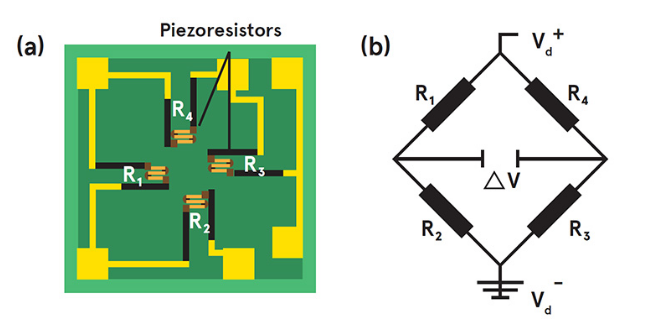
\includegraphics[width=0.7\textwidth]{img/barometro_wheatstone.png}
%     \caption{Puente de Wheatstone conformado por los resistores del sensor de presión. La imagen se extrajo de \cite{baro_3}.}
%     \label{fig:barometro_wheatstone}
% \end{figure}

% \begin{subequations}
%     \begin{align}
%         \Delta V &= (V_d^+ - V_d^-) \left[ \frac{R_2}{R_2 + R_1} - \frac{R_3}{R_3 + R_4} \right]\\
%         R_1 &= R_3 = R - \Delta R\\
%         R_2 &= R_4 = R + \Delta R\\
%         \Delta V &= (V_d^+ - V_d^-) \frac{\Delta R}{R}
%     \end{align}
%     \label{eq:barometro_wheatstone}
% \end{subequations}

% En la aplicación del vehículo aéreo, el barómetro se utiliza con el fin de medir la altura del vehículo, respecto de una altura inicial. La forma de medir la altitud a través de la presión es utilizando la ecuación de los gases nobles para el aire \cite{cavcar2000international}. En las ecuaciones \eqref{eq:gases_nobles} se obtiene una expresión para la presión, en función de la densidad del aire, la constantes de los gases y la masa molar del aire.

% \begin{subequations}
%     \begin{align}
%         P V &= n R T\\
%         n &= \frac{m}{M}\\
%         P V &= \frac{m}{M} R T\\
%         P &= \frac{m}{V} \frac{R T}{M}\\
%         P &= \rho \frac{R T}{M} \label{eq:presion_gas_nobles}
%     \end{align}
%     \label{eq:gases_nobles}
% \end{subequations}

% Luego, utilizando la condición hidrostática, la presión es la ejercida por la columna de aire \cite{cavcar2000international}. En la condición hidrostática de la ecuación \ref{eq:condicion_hidrostatica} se puede despejar la densidad del aire y reemplazarla en \eqref{eq:presion_gas_nobles}. Finalmente, se obtiene la ecuación diferencial de \eqref{eq:presion_diferencial}.

% \begin{equation}
%     dp = -\rho g dh
%     \label{eq:condicion_hidrostatica}
% \end{equation}

% \begin{equation}
%     \frac{dP}{P} = - \frac{g M}{R T} dh
%     \label{eq:presion_diferencial}
% \end{equation}

% Esta ecuación puede integrarse a ambos lados para hallar la relación entre la presión y la altura. Todos los términos de la ecuación \eqref{eq:presion_diferencial} son constantes, a excepción de la temperatura. Según el modelo \textit{International Standard Atmosphere} (ISA), se modela la relación entre la temperatura y la altitud, según la ecuación \eqref{eq:ISA_temperatura}. Esta relación es válida solamente hasta la estratósfera.

% \begin{subequations}
%     \begin{align}
%         T(h) &= T_0 + L \ h\\
%         T(h) &= 288.15 K - h \ 6.5 \ 10^{-3} m/K
%     \end{align}
%     \label{eq:ISA_temperatura}
% \end{subequations}

% Finalmente, se obtiene una expresión de la presión en función de la altura, ecuación \eqref{eq:ISA_presion}. 

% \begin{subequations}
%     \begin{align}
%         P(h) &= P_0 \left[ 1 + \frac{L h}{T_0} \right]^{-\frac{M g}{R L}}\\
%         P(h) &= 1013.25 \ hPa \left[ 1 - 0.0065 \frac{h}{288.15 K} \right]^{5.2561}
%     \end{align}
%     \label{eq:ISA_presion}
% \end{subequations}

% Se puede obtener un modelo más simplificado si se asume una temperatura constante, independiente de la altitud. Se reemplaza en \eqref{eq:presion_diferencial} y resolviendo la ecuación diferencial se obtiene la ecuación \eqref{eq:presion_temp_constante}.

% \begin{subequations}
%     \begin{align}
%         P(h) &= P_0 \ e^{-\frac{g M h}{R T}}\\
%         P(h) &= 1013.25 \ hPa \ e^{-\frac{h}{8840.2 m} }
%     \end{align}
%     \label{eq:presion_temp_constante}
% \end{subequations}

Al igual que con el sensor IMU, se hizo una búsqueda de las distintas alternativas. Los parámetros típicamente especificados son los siguientes:

\begin{itemize}
    \item \textit{Full-scale range}
    \item \textit{Absolute Accuracy}
    \item \textit{Relative Accuracy}
    \item \textit{Solder Drift}
    \item \textit{Offset vs temp}
    \item \textit{Offset vs time}
    \item \textit{Noise}
\end{itemize}

Como se puede ver, estos son similares a los de la IMU. Las diferencias se encuentran en los parámetros \textit{Absolute Accuracy}, \textit{Relative Accuracy} y \textit{Solder Drift}.\\

Se puede plantear un mismo modelo de medición según la ecuación \ref{eq:medicion_vs_real} pero para la presión.

\begin{equation}
    P_m = (1+S)P + P_b(t) + \eta
    \label{eq:medicion_presion}
\end{equation}

En el caso de la IMU, el parámetro \textit{scale factor error} se refiere al término $S$ y el \textit{offset} al término $P_b$. En el caso del barómetro, estos valores se encuentran especificados de otra manera. Si se quiere medir una presión $P$, el error de medición será $\Delta P = S \ P + P_b(t) + \eta$. El término $S \ P + P_b(t)$ corresponde al parámetro \textit{absolute accuracy} \cite{baro_4}. Este error es introducido debido a que la cavidad dentro del sensor no se encuentra a presión 0 perfecta, sino que a un pequeño valor \cite{baro_1}. Por otro lado, el término $S \ P$ se lo denomina \textit{relative accuracy}. Este hace referencia a mediciones diferenciales de presión. Algunos barómetros MEMS traen consigo una funcionalidad para realizar una compensación de offset. Esto dejaría como parámetro de interés para mediciones de presión a la \textit{relative accuracy}, la cual hace referencia al error introducido para mediciones de variaciones de presión.\\

El parámetro \textit{solder drfit} se refiere al offset que se introduce por el propio proceso de soldadura \cite{baro_4}. Este offset también puede ser compensado a través de la calibración del barómetro.\\

Se buscaron modelos de barómetros de distintos fabricantes, para comparar características, teniendo en cuenta la accesibilidad y el bajo costo. En la tabla \ref{tab:comparacion_baros} se muestra una comparación de los distintos barómetros considerados. Sumado a esto, se tuvo en consideración otro aspecto que fue mencionado anteriormente, la longevidad del componente.

\begin{table}[H]
    \centering
    \begin{tabular}{|c||c|c|c|c|c|c|}
        \hline
          & BMP390 & BMP581 & ICP-20100 & LPS22HH & ILPS22QSTR & DPS368\\
        \hline
        Full scale range [hPa] & 300 - 1250 & 300 - 1250 & 260 - 1260 & 260 - 1260 & \cellcolor{green!25}\makecell{260 - 1260 \\ 260 - 4060} & 300 - 1200\\ 
        absolute acc [hPa] & $\pm 0.5$ & $\pm 0.3$ & \cellcolor{green!25}$\pm 0.2$ & $\pm 0.5$ & $\pm 0.5$ & $\pm 1$\\
        realtive acc [hPa] & $\pm 0.03$ & $\pm 0.06$ & \cellcolor{green!25}$\pm 0.01$ & $\pm 0.025$ & $\pm 0.015$ & $\pm 0.06$\\
        \hline
        longevidad & N/A & N/A & N/A & N/A & \cellcolor{green!25}\makecell{10 años \\ enero 2023} & N/A \\
        \hline
        %AEC-Q100 & No & No & No & No & No & No\\
        %\hline       
    \end{tabular}
    \caption{Se muestra la comparación de las distintas alternativas que fueron tenidas en cuenta para la selección del sensor.}
    \label{tab:comparacion_baros}
\end{table}

Las dos alternativas que se evaluaron son los sensores ICP-20100 y el ILPS22QSTR. El primero de ellos presenta las \textit{absolute accuracy} y \textit{relative accuracy} más bajas de entre todas las opciones evaluadas. El sensor ILPS22QSTR presenta características similares y además tiene la particularidad de que el fabricante garantiza su fabricación por 10 años, hasta enero de 2033 \cite{baro_5}. Finalmente el sensor seleccionado fue este último.

En este caso también se tomó como guía el circuito de la hoja de datos del componente. La interfaz de comunicación seleccionada es I2C. Se prefiere utilizar I2C en lugar de SPI ya que puede aprovecharse el uso del mismo bus al que se conecta el barómetro, para conectar otros sensores y dispositivos. De esta manera, se ahorra la cantidad de pistas y conexiones en el diseño del PCB. Si bien I2C tiene un funcionamiento más lento que SPI, las mediciones del barómetro no son tan críticas como las de la IMU. Este sensor, a diferencia de la IMU, no cuenta con una línea de interrupción, por lo que los datos deben obtenerse por \textit{polling} de forma peródica. El circuito completo puede encontrarse en el \nameref{appendix:circuito_esquematico}.

\subsubsection{Magnetómetro}
%\subsection{Magnetómetro}

El magnetómetro es otro de los sensores complementarios al INS. Este se utiliza para obtener estimaciones del ángulo de \textit{yaw} del vehículo, a partir de mediciones del campo magnético terrestre. Estas mediciones son relativas a una terna solidaria al sensor. Esto se muestra en la figura  . Luego el ángulo de \textit{yaw} puede obtenerse a partir del ángulo entre las componentes en $H_y$ y $H_x$.

\textbf{{\color{red} AGREGAR UNA IMAGEN DEL CAMPO MAGNÉTICO MEDIDO POR EL MAGNETÓMETRO CON SUS COMPONENTES}}

Para medir las componentes del campo magnético, el sensor utiliza una serie de materiales resistivos que son sensibles al campo magnético aplicado sobre estos. Se colocan 4 resistores en configuración puente de Wheatstone y se estiman las componentes del campo magnético a partir del desbalance de este.

Para la selección del componente se hicieron comparaciones de las características de varias alternativas. Los parámetros típicamente especificados para el magnetómetro son los siguientes:

\begin{itemize}
    \item \textit{Full-scale range}
    \item \textit{Scale Factor Error}
    \item \textit{Scale Factor Error vs Temp}
    \item \textit{Offset}
    \item \textit{Offset vs temp}
    \item \textit{Noise}
\end{itemize}

Se buscaron modelos de magnetómetros disponibles. Al igual que con el resto de componentes, se redujo la búsqueda a aquellos que sean de bajo costo. En la tabla  se muestra una comparativa de los modelos considerados para la selección final.

\begin{table}[H]
    \centering
    \begin{tabular}{|c||c|c|c|c|}
        \hline
          & HMC5883L & BMM150 & RM3100 & MMC5983MA\\
        \hline
        %Full scale range [uT] & \makecell{$\pm$88;130;190;250;\\400;470;560;810} & \makecell{x,y: $\pm$1200;\\z: $\pm$2000} & $\pm$800 & $\pm$800\\
        Scale Factor Error & $\pm$0,1 \% @ $\pm$200 uT & 1\% & $\pm$0,5\% @ $\pm$200 uT & \cellcolor{green!25}0,1\% @ $\pm$400uT\\
        \hline
        \makecell{Scale Factor Error\\Over Temp} & \makecell{0.3\%/C \\@ -40°C - 125 °C} & N/A & N/A & \cellcolor{green!25}\makecell{0.07 \%/°C \\@ -40°C - 105°C}\\
        \hline
        Offset @25°C & N/A & \cellcolor{green!25}$\pm$ 40 uT & N/A & $\pm$50 uT\\
        \hline
        Offset Over Temp & N/A & N/A & N/A & \cellcolor{green!25}\makecell{$\pm$2nT/°C \\@ -40°C - 105°C}\\
        \hline
        Noise & \makecell{200 nT \\@ FSR = $\pm$88 uT} & \makecell{300 nT @ 25°C,\\ ODR = 20 Hz} & \cellcolor{green!25}30 nT & \makecell{40nT @ ODR = 50 Hz\\60 nT @ ODR = 100 Hz\\80 nT @ ODR = 200 Hz\\120 nT @ ODR = 400 Hz}\\
        \hline
        AEC-Q100 & No & No & No & \cellcolor{green!25}Sí\\
        \hline
    \end{tabular}
    \caption{Se muestra la comparación de las distintas alternativas que fueron tenidas en cuenta para la selección del magnetómetro. En verde se destaca el modelo con las mejores prestaciones para cada especificación.}
    \label{tab:comparacion_mags}
\end{table}

El modelo RM3100 es el que posee el nivel más bajo de ruido. Este componente se utiliza en computadoras de vuelo comerciales, pero además fue utilizado con éxito en el proyceto Artemis de la NASA. A pesar de las bondades que ofrece, el costo de este componente en el momento de la selección era entre 5 a 10 veces superior con respecto a los otros. Finalmente el sensor elegido fue el modelo MMC5983MA. Este es el único de todas las alternativas consideradas que contiene información de todos los parámetros. Además de tener unas muy buenas características, el mismo es de grado automotriz, lo que le da todavía más robustez.

El efecto del campo magnético producido por los motores del UAV afectan las mediciones del sensor, volviéndolo prácticamente inutilizable para la navegación del vehículo. Para evitar este problema, el magnetómetro se montará en una posición elevada respecto de la computadora de vuelo. Esto quiere decir que este sensor no se montará sobre la placa, sino que se conectará como un sensor externo, utilizando alguno de los concetores de la placa.

\subsubsection{Interfaz de Comunicación CAN}
%\subsection{Interfaz de Comunicación CAN}

% Como fue mencionado, la computadora de vuelo cuenta con la capacidad de conexión a un bus CAN. La especificación original del protocolo \cite{specification1991bosch} incluye dentro de sus definiciones, la capa física. Cada nodo de un bus CAN se conecta a este a través de 2 cables, los cuales llevan la señal diferencial. Esto se muestra en la figura \ref{fig:conxeion_al_bus_CAN}. Todo el bus CAN se compone de 2 cables que llevan los mensajes a todos los nodos de la red. Esto es así debido a que el bus CAN originalmente fue diseñado para utilizarse en automóviles y reemplazar la enorme cantidad de conexiones entre módulos. El hecho de que se trate de una señal diferencial hace que la comunicación sea robusta, reduciendo las emisiones electromagnéticas generadas por este. A su vez, es común que el bus sea cableado como un par trenzado, lo que atenúa señales de modo común, producto de cualquier acoplamiento. 

% \begin{figure}[H]
%     \centering
%     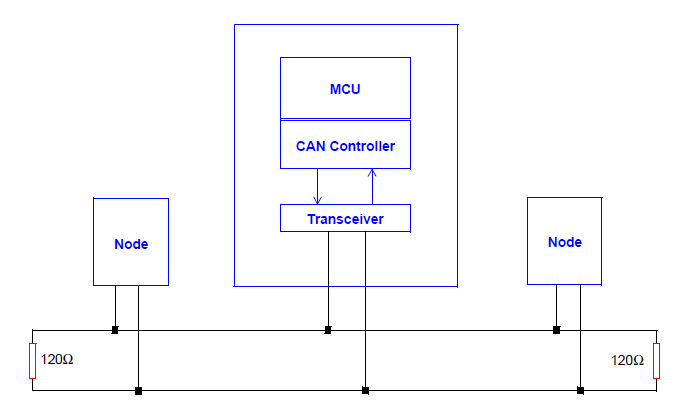
\includegraphics[width=0.5\textwidth]{img/conxeion_al_bus_CAN.png}
%     \caption{La conexión de un nodo al bus es a través de 2 cables que llevan dos señales, CAN-H y CAN-L. La imagen se extrajo de \cite{AN228}.}
%     \label{fig:conxeion_al_bus_CAN}    
% \end{figure}

% Existen muchas versiones del protocolo CAN, en este trabajo se utiliza la versión CAN High Speed. Esta define una velocidad máxima de transferencia de 1 Mbps, para un bus de hasta 40 m de longitud y 30 nodos conectados al mismo bus. Se recomienda que la conexión entre cada nodo y el bus no sea de más de 30 cm. El hecho de poder tener hasta 30 nodos expande las posibilidades de uso del bus, más allá de ser el medio principal de comunicación utilizado para el sistema redundante. Por ejemplo, distintos sensores o incluso actuadores como los motores del vehículo podrían conectarse al bus. {\color{red} Acá tendría que agregar alguna referencia a este uso del bus CAN}.\\

% La impedancia característica del bus debe ser de $120 \ \Omega$. Es común agregar resistores de terminación en ambos extremos, para evitar reflexiones. En algunos casos pueden llegar a encontrarse aplicaciones donde los resistores de terminación se incluyen dentro de alguno de los nodos del bus. Esto no es recomendable, ya que si este se desconecta de forma accidental del bus, todas las comunicaciones entre los demás nodos se verán perjudicadas. Este es el motivo por el cual la computadora de vuelo no incluye este resistor en el circuito.\\

% En la figura \ref{fig:conxeion_al_bus_CAN} se muestran 2 elementos que forman parte del nodo, el \textit{trasnciever} y el \textit{controller}. El primero de ellos forma parte de la capa física y es un circuito que convierte las señales diferenciales del bus en señales de modo común, que luego son transferidas al elemento \textit{controller}. Este componente sirve como interfaz física con el bus.\\

Como ya fue mencionado, la computadora de vuelo requiere que la comunicación entre sus réplicas sea través de un bus. Para ello, la placa debe contar con un circuito con una interfaz de comunicación con el mismo. A partir de lo presentado hasta aquí, el único requerimiento es el método de acceso al medio, el cual debe ser controlado por el tiempo. Teniendo en cuenta que se trata de un trabajo realizado con componentes COTS, el hardware a utilizar debe ser de fácil acceso y con costos razonables. Para el desarrollo de este trabajo, se seleccionó el bus \textit{Controller Area Network} (CAN)\cite{specification1991bosch}. Si bien su método de acceso al medio no es TDMA, existe una extensión del protocolo que justamente busca incorporar esta funcionalidad en otra capa superior.

%En las secciones siguientes se explica un inconveniente, en cuanto a la selección del microcontrolador. 

%El microcontrolador que se utiliza cuenta con un periférico que permite utilizar una interfaz con este bus. A continuación se presentan brevemente algunas características.

%Si bien el método de acceso al medio no es TDMA, existe una extensión del protocolo que justamente busca incorporar esta funcionalidad en otra capa superior.

%\subsubsection{Descripción del Protocolo CAN}

El protocolo CAN fue desarrollado para ser usado en la industria automotriz, como bus de comunicación que conecta distintos módulos dentro de un automóvil. El objetivo de su desarrollo fue similiar al motivo por el cual se desarrolló el bus ARINC 629 en aviones, reemplazar la gran cantidad de cables dentro del vehículo por un bus simple. El protocolo se corresponde con el modelo OSI y la especificación original define las capas física y de enlace.

A diferencia de otros protocolos típicos en sistemas embebidos como I2C o SPI, el protocolo CAN no tiene el formato maestro-esclavo. La comunicación se da entre miembros del bus denominados nodos, los cuales se encuentran conectados a los mismos 2 cables. Esto se muestra en la figura \ref{fig:red_CAN_2}. 

\begin{figure}[H]
    \centering
    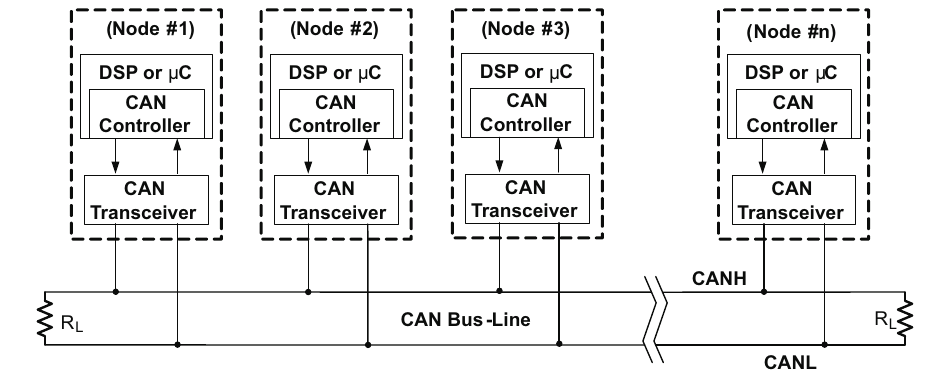
\includegraphics[width=\textwidth]{img/red_CAN.png}
    \caption{Todos los nodos se encuentran conectados al mismo bus de comunicaciones. El bus CAN se compone de dos cables, CAN-H y CAN-L, terminados en sus extremos por resistencias de adaptación. La imagen se extrajo de \cite{texasSLOA101B}.}
    \label{fig:red_CAN_2}
\end{figure}

La impedancia característica del bus debe ser de $120 \ \Omega$. Es común agregar resistores de terminación en ambos extremos, para evitar reflexiones. En algunos casos pueden llegar a encontrarse aplicaciones donde los resistores de terminación se incluyen dentro de alguno de los nodos del bus. Esto no es recomendable, ya que si el mismo se desconecta de forma accidental del bus, todas las comunicaciones entre los demás nodos se verán perjudicadas debido a la pérdida del resistor de adaptación.

La información enviada por los nodos a través de estos 2 cables es en formato de señal diferencial, lo que vuelve robusta a la comunicación, reduciendo las emisiones electromagnéticas generadas por este. A su vez, es común que el bus sea cableado como un par trenzado, lo que atenúa señales de modo común, producto de cualquier acoplamiento.

\textbf{{\color{red} AGREGAR UNA IMAGEN DE OCSILOCSOPIO DONDE SE VEAN LAS SEÑALES DIFERENCIALES DE CAN.}}

El protocolo CAN define dos estados para el bus, \textit{recessive} y \textit{dominant}. Cuando no hay actividad en el bus, tanto la línea de CAN-H como la de CAN-L se encuentran a la misma tensión constante. Esto corresponde al estado \textit{recessive} y equivale a un 1 lógico. Cuando se quiere enviar un 0 lógico, el transciever del nodo transmisor fija la tensión de las líneas CAN-H y CAN-L de tal forma de generar una tensión diferencial $V_{CAN-H} - V_{CAN-L} \geq 1,5 V$. Esto se muestra en la figura \ref{fig:CAN_recessive_dominant}.

\begin{figure}[H]
    \centering
    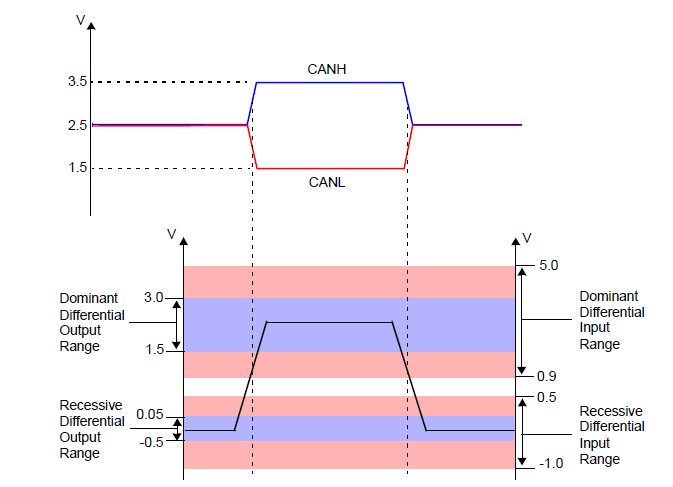
\includegraphics[width=0.7\textwidth]{img/CAN_recessive_dominant.png}
    \caption{Se muestran los estados recessive y dominant del bus CAN y sus equivalentes lógicos.}
    \label{fig:CAN_recessive_dominant}    
\end{figure}

Los nodos solamente actúan sobre el bus cuando quieren fijar un estado \textit{dominant}. Cuando se quiere fijar un estado \textit{recessive}, no se actúa sobre el bus ya que este es su estado por defecto. Esto permite que varios nodos puedan actuar al mismo tiempo. En caso de que esto suceda, el estado \textit{dominant} (de allí su nombre) predominará sobre el estado \textit{recessive}.

Existen muchas versiones del protocolo CAN, en este trabajo se utiliza la versión CAN High Speed. Esta define una velocidad máxima de transferencia de 1 Mbps, para un bus de hasta 40 m de longitud y 30 nodos conectados. Se recomienda que la conexión entre cada nodo y el bus no sea de más de 30 cm. El hecho de poder contar con hasta 30 nodos expande las posibilidades de uso, más allá de ser el medio principal de comunicación utilizado para el sistema redundante. Por ejemplo, distintos sensores o incluso actuadores como los motores del vehículo podrían conectarse al bus. {\color{red} Acá tendría que agregar alguna referencia a este uso del bus CAN}.

%Cada nodo de un bus CAN se conecta a este a través de 2 cables, los cuales llevan la señal diferencial. Esto se muestra en la figura \ref{fig:conxeion_al_bus_CAN}. Todo el bus CAN se compone de 2 cables que llevan los mensajes a todos los nodos de la red. 

% \begin{figure}[H]
%     \centering
%     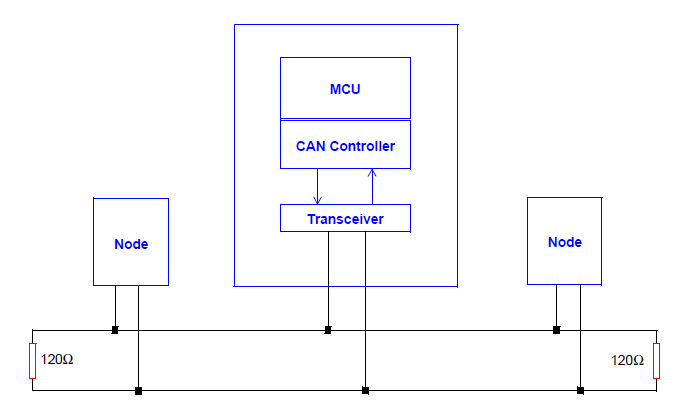
\includegraphics[width=0.5\textwidth]{img/conxeion_al_bus_CAN.png}
%     \caption{La conexión de un nodo al bus es a través de 2 cables que llevan dos señales, CAN-H y CAN-L. La imagen se extrajo de \cite{AN228}.}
%     \label{fig:conxeion_al_bus_CAN}    
% \end{figure}

%Existen muchas versiones del protocolo CAN, en este trabajo se utiliza la versión CAN High Speed. Esta define una velocidad máxima de transferencia de 1 Mbps, para un bus de hasta 40 m de longitud y 30 nodos conectados al mismo bus. Se recomienda que la conexión entre cada nodo y el bus no sea de más de 30 cm. El hecho de poder tener hasta 30 nodos expande las posibilidades de uso del bus, más allá de ser el medio principal de comunicación utilizado para el sistema redundante. Por ejemplo, distintos sensores o incluso actuadores como los motores del vehículo podrían conectarse al bus. {\color{red} Acá tendría que agregar alguna referencia a este uso del bus CAN}.\\

En la figura \ref{fig:red_CAN_2} se muestra que cada nodo se compone de 2 elementos, el \textit{trasnciever} y el \textit{controller}. El primero de ellos forma parte de la capa física y es un circuito que convierte las señales diferenciales del bus en señales de modo común. Luego las señales de modo común son transferidas al elemento \textit{controller}. Este típicamente se encuentra implementado en hardware dentro de una unidad de procesamiento como un microcontrolador, como es el caso de este trabajo.

%En la figura \ref{fig:red_CAN_2} se muestran 2 elementos que forman parte del nodo, el \textit{trasnciever} y el \textit{controller}. El primero de ellos forma parte de la capa física y es un circuito que convierte las señales diferenciales del bus en señales de modo común, que luego son transferidas al elemento \textit{controller}. Este componente sirve como interfaz física con el bus.\\

% Formato de la tama CAN

Una trama del protocolo CAN se comopone de varios campos. Además, se definen 2 tipos de tramas, estándar, figura \ref{fig:CAN_frame_standard} y extended, figura \ref{fig:CAN_frame_extended}.

\begin{figure}[H]
    \centering
    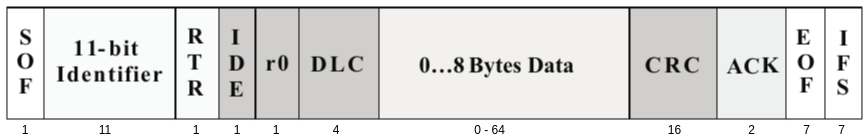
\includegraphics[width=0.8\textwidth]{img/CAN_frame_standard.png}
    \caption{Se muestran los campos de una trama CAN estándar. Debajo de cada campo se indica la cantidad de bits. La imagen se extrajo de \cite{texasSLOA101B}.}
    \label{fig:CAN_frame_standard}
\end{figure}

\begin{itemize}
    \item SOF: Inicio de una nueva trama en el bus.
    \item Identifier: Indica el contenido del campo de datos.
    \item RTR: Dominante para \textit{data frames}, recessive para \textit{remote frames}. Estas últimas se utilizan para solicitar a otro nodo que envíe determinado mensaje. Su formato es el mismo, solo que no pueden contener bytes en su campo de datos.
    \item IDE: Si es dominante, se trata de una trama estándar. Si no, es una trama extended.
    \item r0: Reservado.
    \item DLC: Cantidad de bytes de datos enviados.
    \item Data: Datos útiles, entre 0 y 8 bytes.
    \item CRC: Chequeo de la integridad del mensaje de la trama.
    \item ACK: Se compone de 2 bits denominados ACK SLOT Y ACK DELIMITER. El emisor deja estos campos en recessive y cuando algún nodo recibe el mensaje, fuerza un nivel dominant en el bus, indicando que se recibió el mensaje correctamente.
    \item EOF: Fin de trama.
    \item IFS: Espacio antes de enviar la próxima trama, de 7 bits. 
\end{itemize}

\begin{figure}[H]
    \centering
    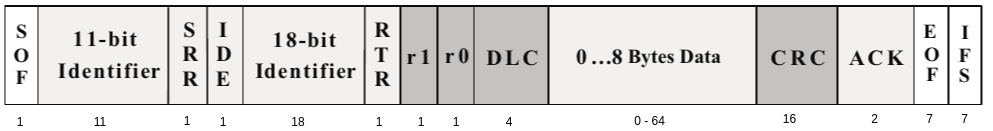
\includegraphics[width=0.8\textwidth]{img/CAN_frame_extended.png}
    \caption{Se muestran los campos de una trama CAN extendida. Debajo de cada campo se indica la cantidad de bits. La imagen se extrajo de \cite{texasSLOA101B}.}
    \label{fig:CAN_frame_extended}
\end{figure}

La trama extended mantiene los mismos campos pero incorpora otros 2 más:

\begin{itemize}
    \item SRR: Debe ser recessive para extended frames.
    \item r1: Reservado.
\end{itemize}

% Acceso al medio


%CAN es un protocolo donde no hay un nodo master, sino que todos pueden utilizar el medio para transmitir mensajes, 
Debido a que no existe un nodo que sea maestro, todos los miembros del bus pueden iniciar la transmisión de un mensaje. El método de acceso al medio se denomina \textit{Carrer Sense Multiple Access with Collision Detection and Arbitration on Message Priority} (CSMA/CD+AMP). Antes de transmitir un mensaje, el nodo sensa el bus y en caso de que esté libre, intenta utilizarlo para transmitir un mensaje.

%En caso de que más de un nodo quiera enviar un mensaje a la vez, esto llevará a una colisión. El protocolo tiene un método para solucionar las colisiones sin tener pérdida de mensajes.

En el eventual caso en que más de un nodo detecte el medio sin uso, estos intentarán transmitir a través del bus al mismo tiempo. Esta situación se encuentra contemplada por el protocolo a través de un mecanismo que resuelve la colisión mientras que asegura la transmisión del mensaje con la prioridad más alta. El mensaje con la prioridad más alta será aquel que tenga en su campo Identifier el valor más bajo. De aquí se desprende la necesidad de que en un mismo bus no haya mensajes distintos con el mismo campo ID.

En la figura \ref{fig:CAN_arbitration} se muestra un ejemplo donde se resuelve una colisión. Tanto el nodo 1 como el nodo 2 quieren utilizar el bus CAN. Ambos comienzan a inyectar su ID correspondiente. En algún momento, ocurre una discrepancia entre el ID inyectado por ambos nodos. Aquel con el campo dominant, es decir 0, gana y completa su transmisión, en este caso el nodo 2. El nodo 1 que quiso enviar un 1 por su lado, detecta un 0. Esto genera que detenga su transmisión, dejando que los demás nodos utilicen el medio.

\begin{figure}[H]
    \centering
    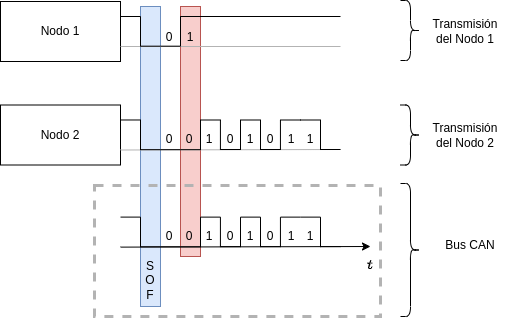
\includegraphics[width=0.6\textwidth]{img/CAN_arbitration.png}
    \caption{Mecanismo para la detección de colisiones. El nodo 2 gana por prioridad y completa su transmisión, mientras que el nodo 1 deja de usar el bus, aguardando a que el nodo 2 finalice.}
    \label{fig:CAN_arbitration}
\end{figure}

%En las figuras \ref{fig:CAN_frame_standard} y \ref{fig:CAN_frame_extended} se puede ver que las tramas tienen un campo CRC, el cual es utilizado para que el receptor pueda verificar la integridad del mensaje. Además, se muestra otro campo, el ACK. Cada vez que un nodo recibe un mensaje correctamente, este sobreescribe el bit de ACK con un dominant, es decir un 0.\\

El protocolo CAN de por sí, no cuenta con un acceso al medio controlado por el tiempo, sino que es dominado por eventos (\textit{event-triggered}), ya que varios nodos pueden iniciar la transmisión de un mensaje en cualquier momento. En el estándar ISO 11898-4\cite{ISO11898_4} se define una extensión del protocolo CAN denominada \textit{Time-Triggered CAN} (TTCAN). Esta justamente fue desarrollada con el objetivo de utilizar el protocolo en aplicaciones de alta confiabilidad. Para ello, TTCAN incorpora un mecanismo de comunicación entre nodos a través de un scheduling estático, el cual es respetado por todos. A cada mensaje del scheduling se le asigna una ventana de tiempo y el mismo se repite de forma periódica.\\

%Al utilizar un scheduling estático, se evitan las colisiones y las retransmisiones. Teniendo en cuenta que se trata de sistemas de alta confiabilidad, una colisión en el bus puede traer consigo el retraso en la transmisión de mensajes críticos para el desempeño del sistema y la seguridad. El scheduling de los mensajes y los tiempos en que estos se envían pasan a formar parte del diseño del sistema.

%Como se mencionó al principio de la sección \ref{sec:requerimentos_sistema_tolerancia_fallas}, la arquitectura para la tolerancia a fallas no está definida. 
%La elección del protocolo CAN le da versatilidad al uso del bus, ya que puede utilizarse con un acceso al medio tanto controlado por el tiempo como por eventos.

%En la figura \ref{fig:microcontrolador_transciever} se muestra la comunicación entre transciever, controller y el bus. Cuando se quiere transferir un mensaje a través del bus CAN, el periférico envía un mensaje a través del terminal CAN TX. El transciever lo recibe y lo convierte en una señal diferencial para inyectarlo en el bus. Cuando el nodo recibe un mensaje del bus CAN, el transciever es el que interactúa con el bus y genera una señal de modo común, la cual es enviada a través del terminal CAN RX al microcontrolador.

% \begin{figure}[H]
%     \centering
%     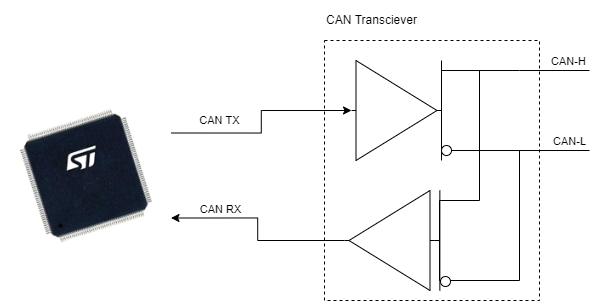
\includegraphics[width=0.5\textwidth]{img/microcontrolador_transciever.png}    
%     \caption{El periférico embebido en el microcontrolador, a través del transciever, puede interactuar con el bus CAN.}
%     \label{fig:microcontrolador_transciever}
% \end{figure}



%La interfaz CAN se compone del transciever, su comunicación con el microcontrolador y el conector.

El micronotrolador seleccionado para la computadora de vuelo, cuenta con 2 \textit{controller} embebido, el periférico bxCAN \cite{STM32F746ZG}. Cada uno de ellos cuenta con 2 líneas de comunicación con el transciever, CAN TX y CAN RX, las cuales se utilizan para enviar y recibir las señales de modo común al \textit{trasnciever}. En cuanto a este útlimo, se trata de un componente que es ampliamente utilizado en la electrónica automotriz, por lo que hay mucha disponibilidad. Existen transcievers que utilizan distintos niveles de tensión en sus salidas. La gran mayoría de los componentes de la computadora de vuelo utilizan tensiones de 3,3 V para su funcionamiento, por lo que se buscó algún componente que pueda trabajar con este nivel de tensión. El componente seleccionado es el SN65HVD230 de Texas Instruments \cite{SN65VHD230}, el cual es compatible con la especificación de capa física de CAN, ISO 11898-2. En la figura \ref{fig:microcontrolador_transciever} se muestra la comunicación del microcontrolador con el bus CAN a través del \textit{transciever}. Este cuenta con una protección por exceso de tempertura, donde el componente pone sus salidas CAN-H y CAN-L en alta impdeancia, de manera de no perturbar al resto de los nodos. Además, cuenta con una funcionalidad que permite detectar si el transciever fue desconectado del bus, fijando un estado alto constante en su salida RX hacia el \textit{controller}, informándole de la situación.

\begin{figure}[H]
    \centering
    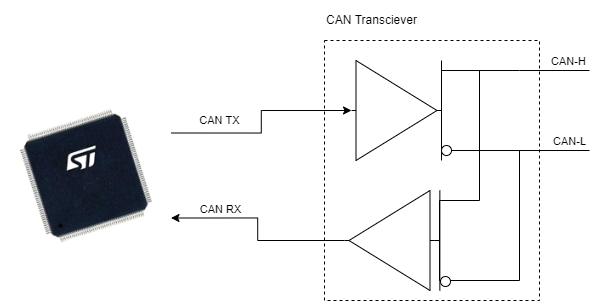
\includegraphics[width=0.5\textwidth]{img/microcontrolador_transciever.png}    
    \caption{Se muestran las conexiones entre el \textit{controller} embebido en el microcontroldaor y el \textit{transciever}, a través de las líneas CAN TX y CAN RX. {\color{red} CAMBIAR ESTA IMAGEN POR UNA MÁS CLARA Y PROLIJA}}
    \label{fig:microcontrolador_transciever}
\end{figure}

Como se muestra en la figura \ref{fig:microcontrolador_transciever}, el \textit{transciever} cuenta con un terminal \textit{Rs} que permite controlar el tiempo de crecimiento y de decrecimiento de las líneas CAN-H y CAN-L. Al realentizar el tiempo de crecimiento en las líneas CAN-H y CAN-L, se atenúa el contenido armónico de las más altas frecuencias, disminuyendo emisiones. Por ejemplo, si se coloca un resistor de $10 \ k\Omega$ en el terminal 8 denominado \textit{Rs}, la hoja de datos indica un slew-rate de $15 \ V / \mu s$.

La especificación de la capa física de CAN no indica un conector a utilizar. Se buscó seleccionar alguno que no ocupe demasiado espacio al ser montado en el PCB. En \cite{CiAconnector} se mencionan algunas recomendaciones de conectores. Este es un documento publicado por la organización internacional sin fines de lucro, \textit{CAN in Automation}, que se dedica a publicar recomendaciones y especificaciones relacionadas al uso del bus CAN. Dentro de las opciones que da este documento, se buscó alguno que tenga dimensiones razonables a lo requerido para la placa. De entre todas las opciones se seleccionó el conector que corresponde a la especificación de un protocolo CAN desarrollado para ser usado en drones, DroneCAN \cite{DroneCAN}, el conector JST GH 4. Por cuestiones de disponibilidad, se seleccionó otro componente similar a este y que es del mismo fabricante de otros de los conectores utilizados para la computadora de vuelo, correspondiente a la serie DF-13 del fabricante Hirose. Este puede ver en la figura \ref{fig:conector_CAN}. Se utilizaron dos de estos conectores, uno por cada \textit{transciever}. Al ser de pequeñas dimensiones, la inclusión de ambos conectores no ocupa demasiado espacio en la placa.

%\textbf{{\color{red} AGREGAR UNA IMAGEN DEL CONECTOR DF13 DE CAN.}}

\begin{figure}[H]
    \centering
    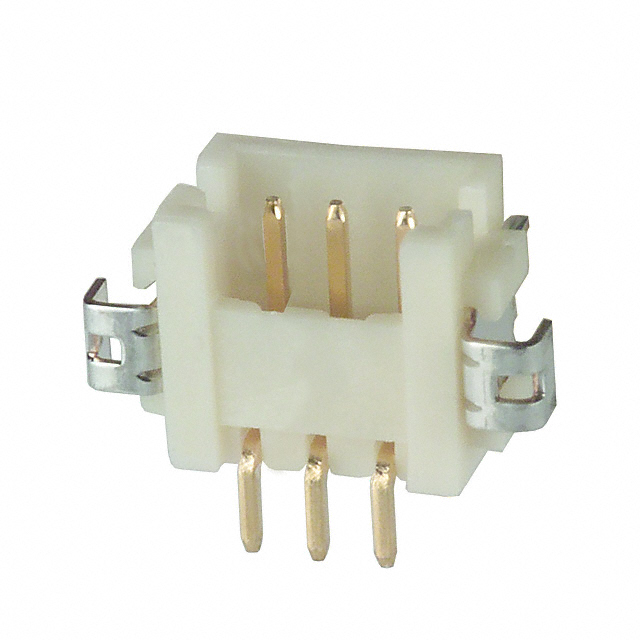
\includegraphics[width=0.2\textwidth]{img/conector_CAN.jpg}    
    \caption{Se muestra el conector utilizado para las interfaces CAN. El mismo cuenta con 3 terminales, de los cuales 2 de se utilizaron para la señal CAN diferencia. El terminal restante corresponde al GND de la placa.}
    \label{fig:conector_CAN}
\end{figure}

En cuanto al circuito implementado, se tomaron como punto de partida las recomendaciones de la hoja de datos del trasnciever SN65HVD230. Este recomienda el agregado de capacitores de desacople en las líneas de alimentación. %Además, se agregaron resistores en serie con las líneas de CAN RX y CAN TX, es decir, en las pistas que llevan las señales que van desde el controller al transciever y viceversa. Esto se hizo como medida preventiva para amortiguar las señales, en caso de que estas presenten sobrepicos en las conmutaciones. A priori se fijan en $0 \ \Omega$ y se modificarán de ser necesario.
El circuito completo de la interfaz CAN puede encontrarse en el \nameref{appendix:circuito_esquematico}.

%\textbf{{\color{red} COMPLETAR EL ANÁLISIS DEL MODELO DE PARÁMETROS CONCENTRADOS, PARA LAS PISTAS CAN-TX Y CAN-RX, PARA CALCULAR EL EVENTUAL RESISTOR EN SERIE.}}

%\subsection{Selección del Bus de Comunicaciones de la Computadora de Vuelo}



\subsubsection{Circuito de Alimentación}\label{sec:circuito_de_alimentacion}
%\subsection{Circuito de Alimentación}

Para alimentar el microcontrolador y los demás componentes, se incluye una fuente de alimentación de $3.3 \ V$. Si bien el uso de una fuente conmutada ofrecería mejores características de eficiencia, se opta por utilizar un circuito con un regulador lineal. El motivo principal es porque se prioriza reducir las dimensiones de la placa y simplificar el diseño. Se incorporó un conector, de manera de poder alimentar la placa utilizando una fuente externa de $5 \ V$, a partir de los cuales se generan los $3.3 \ V$.

%En las primeras dos versiones de la computadora de vuelo, desarrolladas por el LAR en trabajos anteriores, se integró una fuente conmutada de salida $5 \ V$ junto con un regulador lineal de $3.3 \ V$. A partir de la tercera versión, esta fuente conmutada se eliminó dejando solamente el regulador lineal de $3.3 \ V$ \cite{garberoglio2019diseno}. El motivo principal fue reducir las dimensiones de la placa y simplificar el diseño. Siguiendo esta misma línea, la fuente conmutada tampoco se incluyó en este trabajo. Se incorporó un conector, de manera de poder alimentar la placa utilizando una fuente externa de $5 \ V$.

El circuito implementado se comprende del regulador lineal, junto con capacitores de entrada y de salida. Por cuestiones de confiabilidad, se buscó un componente que sea de grado automotriz. Además, se buscó utilizar un encapsulado SOT-223-3, figura \ref{fig:sot_223_3}. Estos componentes son de fácil acceso en el mercado local, lo que facilita el armado final de la placa.

\begin{figure}[H]
    \centering
    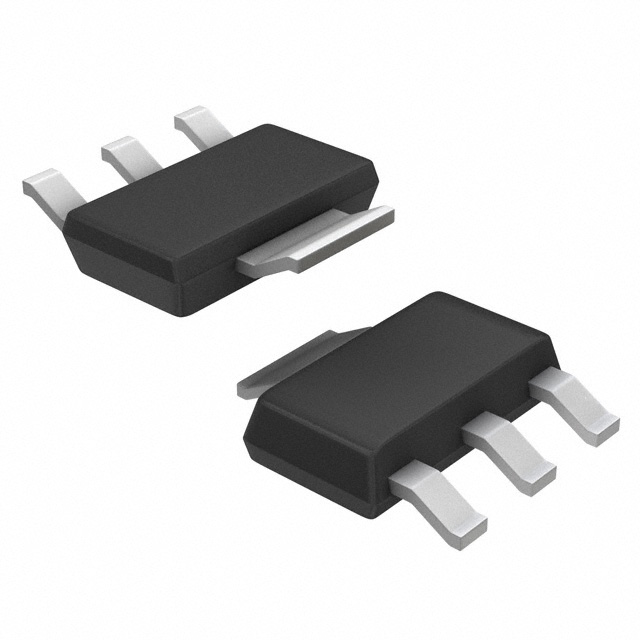
\includegraphics[width=0.3\textwidth]{img/sot_223_3.png}
    \caption{Encapsulado SOT-223-3 seleccionado para el regulador lineal. El terminal de mayor tamaño se encuentra conectado al terminal de tensión de salida, $3.3 \ V$.}
    \label{fig:sot_223_3}
\end{figure}

El modelo seleccionado es el ZLDO1117QG33TA de DIODES Incorporated \cite{ZLDO1117QG33TA}, un regulador low-dropout de grado automotriz con capacidad para entregar hasta 1 A de corriente. Este valor puede resultar excesivo, pero puede ser de utilidad en caso de que sea necesario utilizar muchos módulos y sensores externos a la placa.

Se siguió el circuito recomendado por la hoja de datos del fabricante, donde se coloca un capacitor a la entrada del regulador y otro en su salida. Para el capacitor de entrada se seleccionó un capacitor cerámico multicapa de valor $4.7 \ \mu F$. Estos tienen una ESR muy baja, lo que permite que se descarguen rápido. Esto es importante ya que este capacitor se encargará de proveer corriente al regulador, en caso de que ocurra un escalón en la corriente consumida por la carga. Este capacitor ayuda a mantener la tensión de entrada del regulador, en caso de que la fuente conectada a la entrada del regulador presente un drop-out. 

En cuanto al capacitor de salida, se tuvo en cuenta el hecho de que este es utilizado para la compensación del regulador \cite{TOSHIBALDO}. Al tratarse de un circuito a lazo cerrado, debe asegurar su estabilidad para tener un correcto funcionamiento. El mecanismo de compensación es a través de un compensador en adelanto, formados por dos capacitores de salida $C_o$ y $C_b$, junto con $R_o$, la ESR del capacitor $C_o$. Este compensador incrementa el margen de fase, evitando las respuestas oscilatorias por parte del regulador.

Para compensar el circuito adecuadamente, es importante seleccionar un capacitor $C_o$ con una ESR que no sea ni muy baja ni muy alta \cite{SLVA072}. Para ello, el fabricante recomienda un valor de ESR entre $0.05 \ \Omega$ y $0.5 \  \Omega$, de un valor de por lo menos $4.7 \ \mu F$. Los capacitores MLCC típicamente tienen ESR muy bajas, del orden de unos pocos $m \Omega$. Debido a esto, se selecciona un capacitor de tantalio para el capacitor de salida  $C_o$ \cite{AN1482}. Estos suelen excibir una ESR mayor a la de los MLCC. %El componente seleccionado es el T491A106K016ATAUTO de KEMET.

%Al agregar los capacitores de salida $C_o$ y $C_b$, se forma un compensador en adelanto que incrementa el margen de fase. De este gráfico se desprende que si la resistencia ESR del capacitor de salida $C_o$ es muy pequeña, luego tanto el polo en $1/(C_b R_o)$ como el cero $1/(C_o R_o)$ se desplazan hacia la derecha en frecuencia y no funcionan como compensador en adelanto. Por otro lado, si la ESR es muy grande, el polo y el cero se desplazan a la izquierda y tampoco funcionarán como compensador \cite{SLVA072}. De aquí se desprende el hecho de que la elección del valor de ESR debe ser adecuada.

%En la figura \ref{fig:LDO_diagrama_bloques} se muestra un diagrama en bloques simplificado para un regulador lineal, donde puede verse que se trata de un sistema a lazo cerrado.

%En cuanto al capacitor de salida, este cumple una doble función. Por un lado, aportar a la regulación de línea. Este parámetro es importante teniendo en cuenta que el regulador se utiliza para alimentar un circuito digital, donde aparecen muchas variaciones de corriente. En el caso en el que ocurra un cambio brusco de la corriente de salida del regulador, el capacitor de salida se descargará en parte, para intentar mantener la tensión de salida en un valor constante. 

%Por otro lado, este capacitor también es utilizado para la compensación del regulador \cite{TOSHIBALDO}. En la figura \ref{fig:LDO_diagrama_bloques} se muestra un diagrama en bloques simplificado para un regulador lineal, donde puede verse que se trata de un sistema a lazo cerrado.

% \begin{figure}[H]
%     \centering
%     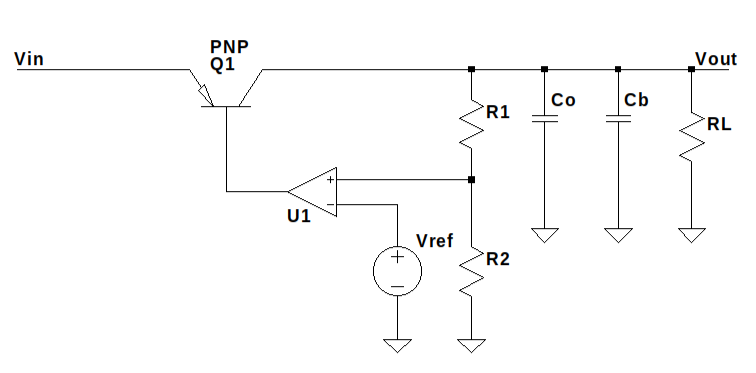
\includegraphics[width=0.7\textwidth]{img/LDO_diagrama_bloques.png}
%     \caption{Diagrama en bloques de un regulador lineal. Este se compone de un transistor de paso, un amplificador de error, una tensión de referencia y un bloque realimentador, formado por $R_1$ y $R_2$. En el diagrama además se muestra $R_L$ que simboliza una carga resistiva y dos capacitores $C_o$ y $C_b$. Estos elementos forman un circuito a lazo cerrado que estabiliza la tensión de salida $V_{out}$.}
%     \label{fig:LDO_diagrama_bloques}    
% \end{figure}

%Para analizar la ganancia de lazo, se plantea el esquema de realimentación en la figura \ref{fig:LDO_esquema_realimentacion}. Para el transistor de paso, se utiliza su modelo de pequeña señal. 

% \begin{figure}[H]
%     \centering
%     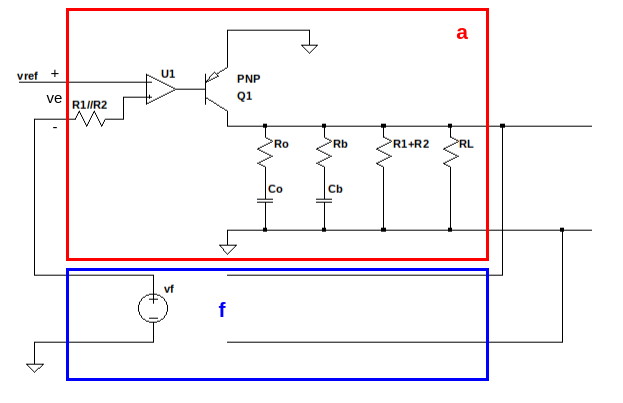
\includegraphics[width=0.8\textwidth]{img/LDO_esquema_realimentacion.png}
%     \caption{Circuito equivalente para analizar la realimentación del regulador lineal. La tensión $v_{in}$ se pasiva ya que se analiza el circuito en el punto de operación.}
%     \label{fig:LDO_esquema_realimentacion}    
% \end{figure}

%Se trata de un esquema que muestrea tensión y suma tensión. El bloque \textit{f} es tal que cumple con la relación de la ecuación \eqref{eq:LDO_bloque_f}. En cuanto al bloque \textit{a}, la transferencia corresponde a la ecuación \eqref{eq:LDO_bloque_a}, donde se ha asumido que $R_b \rightarrow 0$ por ser la ESR de un capacitor cerámico multicapa, $R_L \ll r_o$ y $R_L \ll (R_1+R_2)$. Además, se asume que $R_o \ll R_L$.

% \begin{subequations}
%     \begin{align}
%         v_f &= f \ v_o\\
%         f &= \frac{R_2}{R_1 + R_2} \label{eq:LDO_bloque_f}
%     \end{align}
% \end{subequations}

% \begin{subequations}
%     \begin{align}
%         v_o &= a \ v_{ref}\\
%         a &= A_v(s) g_m  R_L \frac{1 + s C_o R_o}{\left( 1 + s C_o  R_L \right)  \left( 1 + s C_b R_o \right)} \label{eq:LDO_bloque_a}
%     \end{align}
% \end{subequations}

%La transferencia $A_v(s)$ corresponde al amplificador de error y se modela como de un polo simple. Juntando los bloques $a$ y $f$ puede obtenerse la ganancia de lazo para analizar la estabilidad, ecuación \eqref{eq:LDO_ganancia_lazo}. Esta se compone de 3 polos y 1 cero. Este último junto con uno de los polos dependen directamente del valor $R_o$, es decir, la ESR del capacitor de salida $C_o$. En caso de que la ESR sea muy pequeña, se obtiene un sistema con dos polos. Si bien este es estable, su margen de fase es muy pequeño. Esto se traduce en respuestas a transitorios con oscilaciones, por ejemplo causados por variaciones en la corriente de salida del LDO. En la figura \ref{fig:LDO_ganancia_lazo_1} se muestra la comparación entre el sistema compensado y sin compensación.

% \begin{equation}
%     af = \frac{R_2}{R_1+R_2} A_v(s) g_m  R_L \frac{1 + s C_o R_o}{\left( 1 + s C_o R_L \right) \left( 1 + s C_b R_o \right)}
%     \label{eq:LDO_ganancia_lazo}
% \end{equation}

% \begin{figure}[H]
%     \centering
%     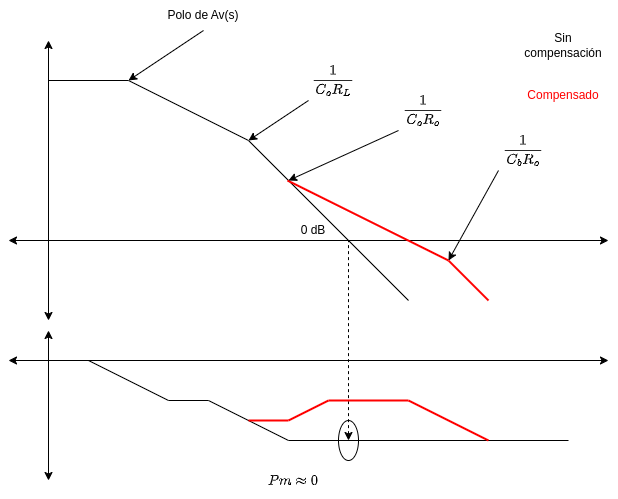
\includegraphics[width=0.7\textwidth]{img/LDO_ganancia_lazo_1.png}
%     \caption{Se muestra un gráfico representativo de la ganancia de lazo de un LDO. En rojo se destaca cómo varía la ganancia de lazo con el agregado de un polo y un cero.}
%     \label{fig:LDO_ganancia_lazo_1}    
% \end{figure}

%Al agregar los capacitores de salida $C_o$ y $C_b$, se forma un compensador en adelanto que incrementa el margen de fase. De este gráfico se desprende que si la resistencia ESR del capacitor de salida $C_o$ es muy pequeña, luego tanto el polo en $1/(C_b R_o)$ como el cero $1/(C_o R_o)$ se desplazan hacia la derecha en frecuencia y no funcionan como compensador en adelanto. Por otro lado, si la ESR es muy grande, el polo y el cero se desplazan a la izquierda y tampoco funcionarán como compensador \cite{SLVA072}. De aquí se desprende el hecho de que la elección del valor de ESR debe ser adecuada.\\

%El fabricante recomienda un valor de ESR entre $0.05 \ \Omega$ y $0.5 \  \Omega$, de un valor de por lo menos $4.7 \ \mu F$. Los capacitores MLCC típicamente tienen ESR muy bajas, del orden de unos pocos $m \Omega$. Debido a esto, se selecciona un capacitor de tantalio para el capacitor de salida \cite{AN1482}, que suelen excibir una ESR mayor a la de los MLCC. El componente seleccionado es el T491A106K016ATAUTO de KEMET. Al igual que Murata, este proveedor ofrece curvas de las características del componente.\\

Como fue ya fue mencionado, se incorpora un conector que permite adosar una fuente externa de $5 \ V$. Este se seleccionó pensando en utilizar algunos módulos típicos para drones y vehículos aéreos \cite{HolybroPM02PowerModule}. Además de las líneas de tensión y de retorno, cuentan con dos señales analógicas que informan acerca de la tensión y la corriente de la batería. La computadora de vuelo sensa dicha información utilizando entradas analógicas. Además, se incluyen dos filtros pasa bajos, uno por cada señal analógica. Estos pueden encontrarse en el \nameref{appendix:circuito_esquematico}.

\subsubsection{Micro SD}

% Por qué se necesita una micro sd
Con el objetivo de registrar datos, tanto del estado como de la misión del vehículo, se incorpora la posibilidad de uso de una memoria Micro SD. Esta permite almacenar una gran cantidad de datos sin procesar, como por ejemplo datos crudos de los sensores del vehículo. Existe una gran variedad de memorias micro SD, las cuales se pueden clasificar según su capacidad:

\begin{itemize}
    \item Standard Capacity SD Memory Card (SDSC): hasta 2 GB.
    \item High Capacity SD Memory Card (SDHC): más de 2 GB, hasta 32 GB.
    \item Extended Capacity SD Memory Card (SDXC): más de 32 GB, hasta 2 TB.
    \item Ultra Capacity SD Memory Card (SDUC): más de 2 TB, hasta 128 TB.
\end{itemize}

% Selección del slot SD

% Circuito implementado
La memoria se compone de una interfaz eléctrica, un controlador interno, una serie de registros y la memoria en sí. Tanto la capa física como el protocolo de comunicación se encuentran definidos en el estándar de la SD Association, ``SD Specifications Part 1 Physical Layer Specifications''. Se definen 2 formas diferentes de comunicación con la memoria, SD Bus y SPI, siendo el primero el que se utiliza en este trabajo.

El protocolo que se define en este estándar tiene el formato master-slave, en este caso el master será el microcontrolador de la computadora de vuelo. En la figura \ref{fig:SD_bus_conexiones} se muestra un esquema con las conexiones entre el master y la memoria.

\begin{figure}[H]
    \centering
    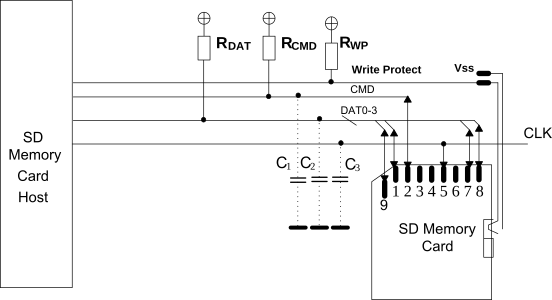
\includegraphics[width=0.8\textwidth]{img/SD_bus_conexiones.png}
    \caption{Esquema circuital de la conexión entre el SD host y una memoria SD, tal y como lo indica la especificación de la SD Association. {\color{red} ESTA IMAGEN NO PUEDE QUEDAR, TENGO QUE DIBUJAR UNA SIMILAR YO}.}
    \label{fig:SD_bus_conexiones}
\end{figure}

El estándar define que la alimentación $V_{dd}$ debe estar entre $2.7 \ V$ y $3.6 \ V$, por lo que puede alimentarse a través del mismo regulador de la placa. A través de la línea CLK, el host envía la señal de clock a la memoria SD para sincronizar la transferencia de datos. La línea CMD es una línea de envío y recepción de comandos, para la lectura de la memoria, escritura, etc. Finalmente, las líneas D0, D1, D2 y D3 se utilizan para envío y recepción de los datos desde y hacia la memoria.

El modo de comunicación SPI permite el uso con microcontroladores de propósito general, los cuales suelen incluir varios periféricos SPI. El uso de este protocolo simplifica la comunicación, aunque como  contrapartida, debido a que el bus SPI tiene una sola línea de datos, las velocidades de transferencia alcanzadas son inferiores. El bus SPI del microcontrolador que se utiliza en este trabajo, tiene una velocidad de transferencia máxima de 6,25 MB/s (50 MHz), mientras que la interfaz SD incluida alcanza velocidades de 25 MB/s (50 MHz). El motivo principal es que el protocolo SD tiene 4 líneas de datos en paralelo, mientras que con el uso de SPI solo se utiliza 1 línea.

% Velocidades de la micro SD
El periférico del microcontrolador es compatible con la versión 2.0 de la SD Association, la cual solamente define las clasificaciones SDSC y SDHC. Además, se aclara que un host que puede comunicarse con una SDHC, también puede comunicarse con una SDSC, pero no al revés. En consecuencia, la computadora de vuelo podrá utilizar tarjetas de hasta 32 GB, correspondientes a las SDHC.

%El periférico del microcontrolador es compatible con La especificación de la SD Association, en su versión 2.0indica que un host que puede comunicarse con una SDHC, también puede comunicarse con una SDSC, pero no al revés. El microcontrolador de la placa cuenta con una interfaz compatible con la versión 2.0 de la SD Association, la cual solamente define las SDSC y SDHC. En consecuencia, la computadora de vuelo solamente podrá utilizar tarjetas de hasta 32 GB, correspondientes a las SDHC.

% Indicar el mecanismo para detectar la SD.
Se coloca un slot para memoria micro SD en la placa, modelo DM3AT-SF-PEJM5 del fabricante Hirose. Además de las líneas de comunicación ya mencionadas, este posee un terminal extra que permite detectar si se insertó una memoria SD. Este terminal funciona como una llave mecánica que se conecta a GND cuando se inserta la memoria en el slot. A través de la conexión con un GPIO del microcontrolador, se puede detectar la inserción de la memoria micro SD, para luego inicializar la comunicación. Al igual que el resto de componentes, el circuito completo puede encontrarse en el \nameref{appendix:circuito_esquematico}.

% Velocidades de la micro SD
%La especificación de la SD Association indica que un host que puede comunicarse con una SDHC, también puede comunicarse con una SDSC, pero no al revés. El microcontrolador de la placa cuenta con una interfaz compatible con la versión 2.0 de la SD Association, la cual solamente define las SDSC y SDHC. En consecuencia, la computadora de vuelo solamente podrá utilizar tarjetas de hasta 32 GB, correspondientes a las SDHC.

%\textbf{{\color{red} COMPLETAR}}

\subsubsection{Interfaz USB}
%\subsection{Interfaz USB}

Como parte de las funcionalidades básicas para utilización de la computadora de vuelo, se incorpora una interfaz para comunicación USB. Este puerto se incorpora con el objetivo de facilitar el uso de la placa durante las etapas de desarrollo de firmware, donde puede ser necesario hacer muchas pruebas y modificaciones. De esta forma, es posible programar la placa y proveer alimentación a través de un solo cable. La interfaz también puede aprovecharse como un puerto de comunicación más con la computadora de vuelo.

El microcontrolador utilizado integra un periférico compatible con la especificación USB 2.0 y con la extensión On-The-Go (OTG), el cual permite a pequeños dispositivos funcionar como hosts en el bus USB. Para las aplicaciones que se le quieren dar a la computadora de vuelo, se opta por un uso de modo device. 

En cuanto a la velocidad de comunicación, el periférico brinda la posibilidad de utilizar tanto una configuración Full-Speed (12 Mb/s) como High-Speed (480 Mb/s). A priori, esta última sería de preferencia, dada la altísima tasa de transferencia, en comparación con la primera. Sin embargo, la utilización de esta última requiere el agregado de un componente adicional para utilizar como interfaz física con el bus USB, denominado ULPI. No sucede lo mismo para el uso de la configuración Full-Speed, para la cual la interfaz física se encuentra completamente integrada. Por una necesidad de mantener un tamaño de placa reducido y teniendo en cuenta que la interfaz USB no se usará para funciones críticas de la computadora de vuelo, se prefirió optar por el uso de una configuración Full-Speed. Cabe aclarar además, que la interfaz física integrada para Full-Speed trae consigo integrado el resistor de pull-up de $1.5 \ k\Omega$ en la línea D+, neceario para el proceso de enumeración del dispositvo, por lo que tampoco fue necesario su incorporación en la placa.

Se incorpora en la placa un conector micro USB-B. El terminal 4 llamado ID se utiliza para indicar si el dispositivo funcionará como host o device. La computadora de vuelo funcionará siempre en modo device, por lo que este se deja en circuito abierto, tal como indica la especificación USB 2.0.

%\textbf{{\color{red} AGREGAR IMAGEN DEL POWER ORING}}

Como fue mencionado, el conector USB se utiliza como otra opción para alimentar la placa. La tensión nominal entregada por un host USB es de $5 \ V$. Para limentar el resto de la placa, se conecta esta entrada al regulador de $3.3 \ V$ que se encuentra en la placa. De forma de evitar que haya conflictos con el conector de alimentación principal mencionado en la sección \ref{sec:circuito_de_alimentacion}, se incorporó un circuito simple formado por dos diodos, como se muestra en la figura \ref{fig:diode_oring}.

\begin{figure}[H]
    \centering
    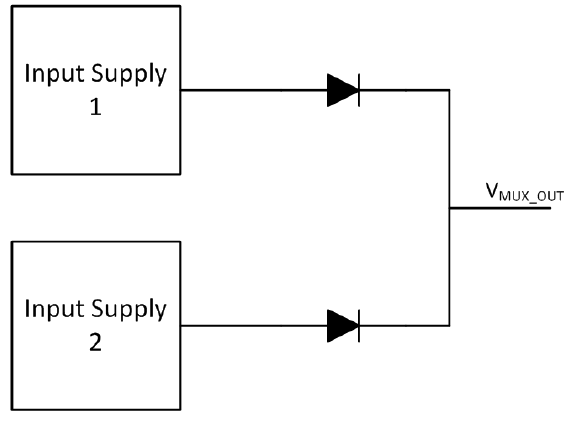
\includegraphics[width=0.4
    \textwidth]{img/diode_oring.png}
    \caption{Se muestra un esquema como el incluido en la computadora de vuelo, el cual permite la aliemntación de la misma a través de 2 fuentes distintas. {\color{red} REEMPLAZAR ESTA IMAGEN POR UNA DIBUJADA POR MI.}}
    \label{fig:diode_oring}    
\end{figure}

Estos diodos fuerzan a que las corrientes solamente fluyan desde las entradas de $5 \ V$ hacia el regulador. Debido a que estos se encuentran en serie con las corrientes de entrada a la placa, se seleccionaron diodos Schottky para tener bajas caídas de tensión, además de reducir la potencia disipada. El circuito completo puede encontrarse en el \nameref{appendix:circuito_esquematico}. Si bien existen componentes especiales que permiten cumplir con esta misma funcionalidad con menor caída de tensión e incluso con la capacidad de seleccionar la fuente de alimentación a utilizar, nuevamente se opta por una solución que permita mantener unas dimensiones reducidas de la placa.

%\textbf{{\color{red} COMPLETAR}}

\subsubsection{Conector para Módulo GPS}
%\subsection{Conector para Módulo GPS}

Se provee la posibilidad de incorporar de forma externa un módulo receptor de GPS. Estos entregan mediciones de posición y velocidad a la computadora de vuelo, los cuales se utilizan como mediciones complementarias al INS. Estos módulos además suelen proveer de una funcionalidad extra, llamada señal \textit{Pulse-per-second}(PPS). Esta es una señal con un período de 1 segundo y que se encuentra sincronizada con los relojes atómicos del sistema GPS, los cuales tienen una exactitud de decenas de ns. Esta señal típicamente es utilizada como referencia de tiempo en el sistema de navegación de la computadora de vuelo.

\begin{figure}[H]
    \centering
    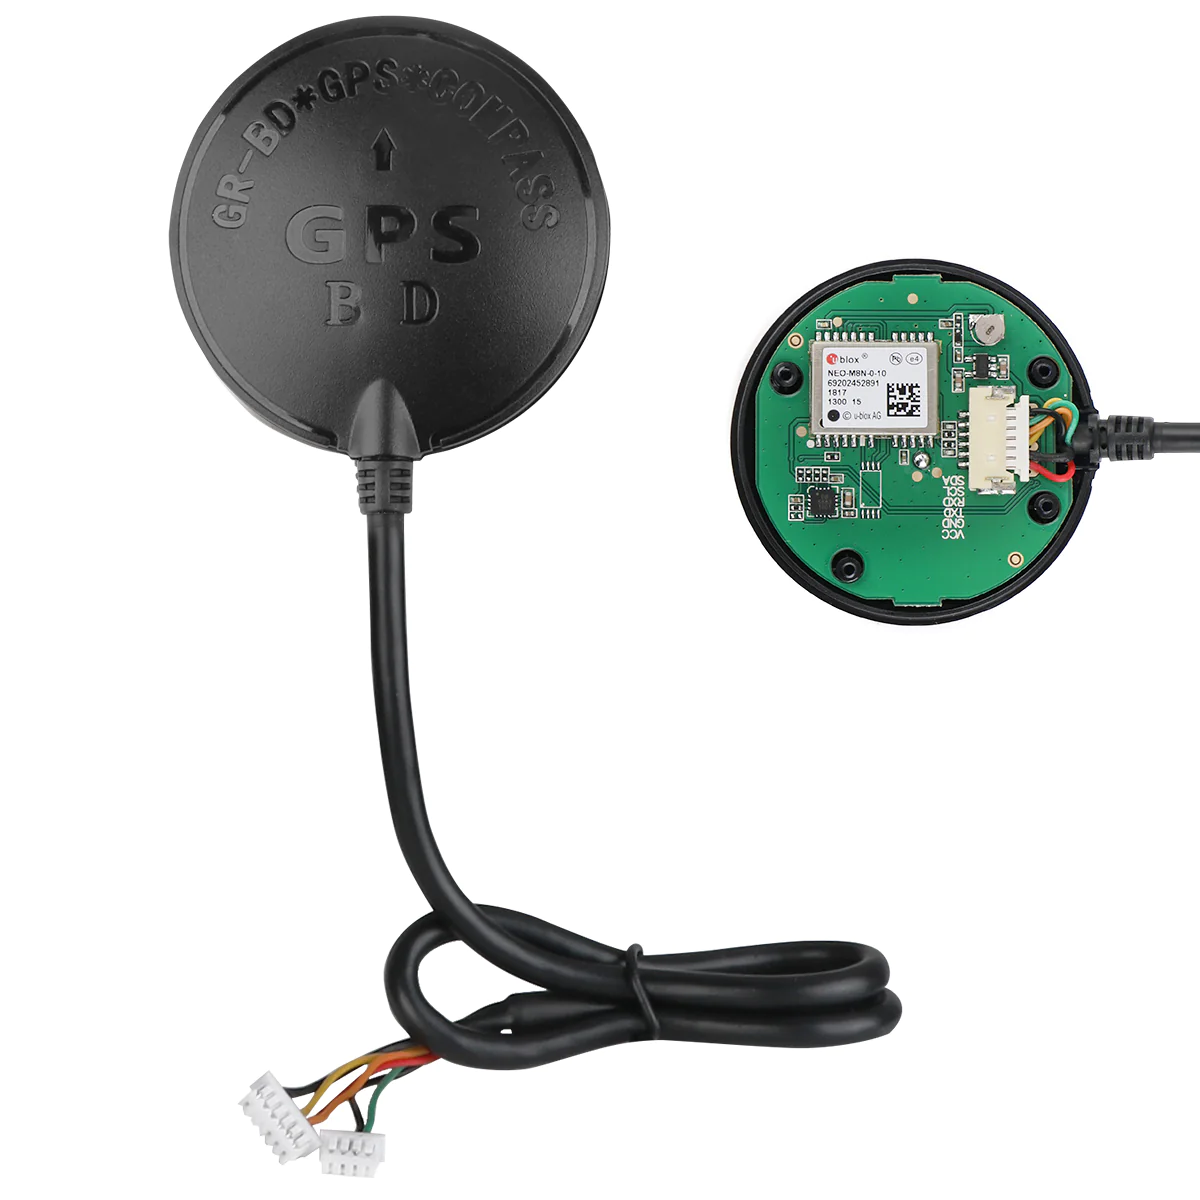
\includegraphics[width=0.5\textwidth]{img/gps.png}
    \caption{Módulo receptor de GPS. Dentro de la carcasa de plástico se encuentra un chip que procesa las señales de GPS para extraer la información, además de una antena utilizada para recibir la señal proveniente de distintos satélites, típicamente una antena parche de cerámica.}
    \label{fig:gps}
\end{figure}

Se proveen de 2 conectores diferentes para uso de este tipo de módulos. Por un lado, se utiliza un conector de la serie DF-13 del fabricante Hirose y por el otro, conectores de tira de pines estándar de 0.1” a 90 grados. En la figura \ref{fig:gps} se muestra un módulo típico de uso en vehículos aéreos de uso comercial, el cual trabaja con una interfaz de comunicación serie. Los conectores incorporados están enfocados al uso de módulos de este tipo, por lo que en el conector pueden verse dos terminales con las etiquetas TX y RX. Estos además están acompañados por un terminal para la señal PPS.

\subsubsection{Conectores para Salidas de PWM}
%\subsection{Conectores para Salidas de PWM}

Como parte del sistema de control, la computadora de vuelo debe comandar a los actuadores. En vehículos aéreos no tripulados comerciales, es común el uso de motores burshless de corriente continua. Estos se alimentan con una fuente de tensión continua, a través de un driver que genera una salida trifásica. Estos drivers se denominan \textit{Electronic Speed Controller}(ESC). 

Haciendo una búsqueda de los distintos tipos de ESC, puede verse que estos ofrecen interfaces de comunicación variadas, siendo la más común el uso de una señal PWM. Es por esto que en la computadora de vuelo se incorpora un conector el cual ofrece 8 salidas para este tipo de señal. Con motivo de tener compatibilidad con drivers comerciales, los conectores incorporados son conectores de tira de pines estándar de 0.1” a 90 grados. Las señales PWM serán generadas a través de los periféricos asociados a los timers del microcontrolador.

\textbf{{\color{red} PONER UNA IMAGEN DONDE SE VEA QUE LA PLACA ENTREGA PWM PERO QUE LA CORRIENTE LA ENTREGA LA BATERÍA}}

Además de las 8 salidas para control de los actuadores del vehículo, se incorporaron otras 4 salidas extra en otro conector separado. Este segundo conector está pensado para utilizarse con otros fines, como controlar una serie de servomotores que puedan incorporarse al vehículo.

%\textbf{{\color{red} COMPLETAR}}

\subsubsection{Conectores para Control por Radio}
%\subsection{Conector para Control por Radio}

%Acá hay que explicar el terminal para DSM Spektrum y el de PPM. Hay que mencionar que son dos formas de comandar a la computadora de vuelo mediante un piloto remoto. Explicar el principio de funcionamiento de cada uno: señales, interfaces, módulos, etc. Finalmente para cada uno hay que explicar el por qué del conector (para DSM spektrum es fácil porque en la especificación dice qué conector usar.)

Como fue mencionado, el vehículo en algunas ocasiones puede ser controlado manualmente por un piloto remoto. Una de las formas de control para vehículos comerciales es a través de un control radio transmisor RC. Estos cuentan con 2 \textit{sticks} a través de los cuales puede guiarse al vehículo manualmente. El movimiento de los \textit{sticks} es interpretado por un circuito que emite las señales moduladas a través de una antena. En el vehículo se monta un receptor, el cual recibe y demodula las señales de radiofrecuencia, para luego entregar los comandos del piloto a la computadora de vuelo.

La forma más común de comunicación entre el receptor y la computadora de vuelo es 
%La forma en la que los receptores comunican los comandos del piloto a la computadora de vuelo puede ser de distintas maneras. La más común de ellas es 
a través de distintas señales del tipo PWM denominadas canales. Cada canal puede indicar un set point distinto del vehículo, por ejemplo pueden tenerse 4 canales para los ángulos \textit{pitch}, \textit{roll}, \textit{yaw} y otro para el empuje vertical del vehículo \cite{garberoglio2019diseno}. Debido a que esto requiere el uso de 4 líneas de comunicación entre el receptor y la computadora de vuelo, se opta por una alternativa similar. %denominada receptor PPM.
Estos utilizan una señal denominada \textit{Pulse Position Modulation} (PPM) y tiene la ventaja de contener la información de todos los canales en una sola línea de comunicación. En la figura \ref{fig:senial_ppm} pueden verse las características de la señal PPM.

\begin{figure}[H]
    \centering
    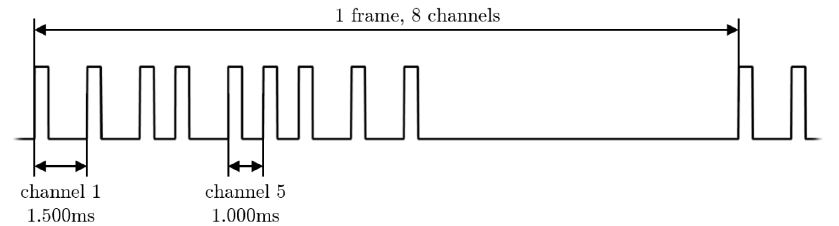
\includegraphics[width=\textwidth]{img/senial_ppm.png}
    \caption{Ejemplo de una señal PPM para 8 canales {\color{red} REEMPLAZAR ESTA IMAGEN POR UNA DIBUJADA POR MI.}.}
    \label{fig:senial_ppm}
\end{figure}

Esta se compone de \textit{frames} de duración 20 ms. En cada \textit{frame} puede haber una cierta cantidad de pulsos de ancho fijo. La información de cada canal se encuentra codificada en el espaciado entre pulsos, el cual puede ser un valor entre $1$ y $2 \ ms$. Un espaciado de $1 \ ms$ representa un valor de 0 \%, mientras que $2 \ ms$, un valor de 100 \%. Estos porcentajes se asocian a los movimientos hechos por el piloto en los \textit{sticks} del radio transmisor. Por ejemplo, en la figura \ref{fig:senial_ppm} el canal 1 tiene una separación entre pulsos de $1.5 \ ms$ (50 \%), mientras que el canal 5, de $1 \ ms$ (0 \%).

En la computadora de vuelo se incluye un conector de tira de pines
estándar de 0.1” a 90 grados de 3 terminales, 2 de ellos para alimentar el módulo desde la computadora de vuelo y el tercero para la comunicación. Para interpretar la señal se utiliza un periférico timer del microcontrolador y se aprovecha la funcionalidad \textit{Input capture mode}. Cada vez que ocurre un flanco, el periférico captura el estado del timer, almacenándolo en un registro auxiliar. Estos valores pueden recuperarse con una interrupción o utilizando DMA. A partir de la diferencia entre valores consecutivos, puede conocerse el espaciado entre pulsos y por ende recuperar el comando enviado por el piloto.

%Un aspecto negativo es que esto requiere el uso de 4 líneas de comunicación entre el receptor y la computadora de vuelo, por lo que se prefiere evitar el uso de estos receptores.


%Se incluye En la placa se incluye un conector para uso de receptores de radio 


Otro de los receptores comúnmente utilizados son los del fabricante Spektrum, denominados \textit{Direct Signal Modulation} (DSM). En lugar de generar una señal modulada, estos utilizan una interfaz UART de comunicación serie. Existe una especificación donde se explica el protocolo, el contenido de los mensajes, velocidades, etc. \cite{Spektrum_spec}. De acuerdo a lo indicado en la especificación, en la computadora de vuelo se incluye un conector modelo B3B-ZR-SM4-TF(LF)(SN) del fabricante JST. 

%\textbf{{\color{red} ESTARÍA BUENO PONER UN DIBUJO EXPLICANDO LA SEÑAL PPM}}

%\textbf{{\color{red} COMPLETAR}}

\subsubsection{Conector para Programación y Debugging por SWD}
%\subsection{Conector para Programación por SWD}

Con el objetivo de facilitar el desarrollo de firmware para distintas aplicaciones, se incorpora un conector con acceso a los terminales de programación y debugging del microcontrolador. Estos corresponden a una interfaz \textit{Serial Wire Debug} (SWD). A través de esta es posible detener el núcleo del microcontrolador utilizando \textit{breakpoints} y examinar el estado de las variables del programa.

%La interfaz SWD permite la comunicación con un dispositivo de debugging compatible con el protocolo. Para su uso se requiere de un terminal de datos bidireccional, SWDIO, además de una línea de clock, SWCLK, generada por el dispostivo de debugging. Esta última se debe a que se trata de una comunicación sincrónica. Algunas interfaces incorporan una tercera línea denominada SWO. Esta es una línea de comunicación asincrónica unidireccional desde el microcontrolador hacia el dispositivo de debugging. SU funcionamiento equivale a una UART y puede usarse para enviar mensajes a una PC, por ejemplo de valores de variables. El uso de este terminal debe acompañarse con un \textit{Serial Wire Viewer} (SWV).

El protocolo necesita el agregado de unos resistores de pull-up y pull-down en las líneas SWDIO y SWCLK respectivamente. En la hoja de datos se indica que estos se encuentran integrados en el microcontrolador, por lo que se hicieron las conexiones desde el microcontrolador directamente hacia un conector utilizado para comunicación con el dispositivo de debugging. No existe un conector estándar para SWD, aunque sí existe una recomendación por parte de ARM, Samtec FTSH 0,050'', tanto de 10 como de 20 terminales \cite{ARM_SWD_connector}. Por motivos de compatibilidad con el debugger disponible en el momento del desarrollo, se optó por un conector más simple, conformado por tiras de pines estándar de 0.1” verticales. En este mismo conector se incorporan líneas de alimentación y GND, permitiendo la alimentación de la placa, además de una línea de reset, la cual puede ser manejada por el debugger.

%\textbf{{\color{red} COMPLETAR}}

%\subsubsection{Micro Switch}
\subsubsection{Otras Funcionalidades}
%\subsection{Micro Switch}

Además del pulsador para la línea de RESET, se incluyen dos pulsadores extra. Estos a priori no tienen una funcionalidad definida, por lo que se incluyen para ser usados según lo requiera la aplicación de la computadora de vuelo.

Una de los posibles usos que se le puede dar a estos pulsadores es el de ejecutar una rutina de calibración de alguno de los sensores, como el magnetómetro externo, el cual se requiere una calibración que involucra un procedimiento manual.

Teniendo presente la necesidad de obtener un diseño de tamaño reducido, se incorporaron pulsadores de 2 terminales, como los que se muestran en la figura \ref{fig:pulsadores}. Cada pulsador se encuentra acompañado de un resistor de pull-up, acompañado de un capacitor de filtrado y un resistor en serie con motivo de filtrar el efecto rebote.

\begin{figure}[H]
    \centering
    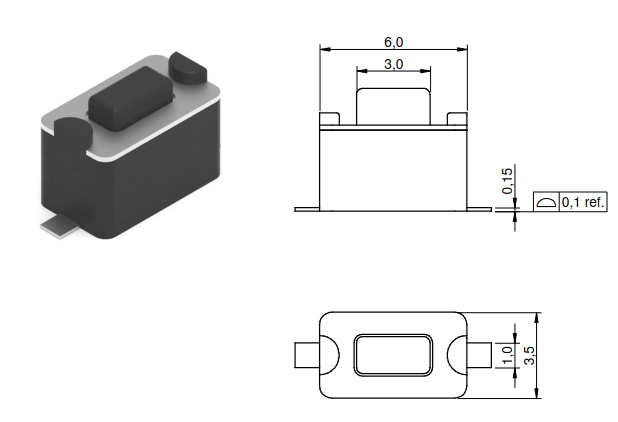
\includegraphics[width=0.5\textwidth]{img/pulsadores.png}
    \caption{Pulsadores utilizados para la computadora de vuelo. Las imágenes se extrajeron de la hoja de datos del componente. Se muestran las dimensiones en mm.}
    \label{fig:pulsadores}    
\end{figure}

%\textbf{{\color{red} COMPLETAR}}

%\subsubsection{LEDs Indicadores}
%\subsection{LEDs Indicadores}

Otra de las funcionalidades que se incorporan son una serie de LEDs de distintos colores. En total se incorporaron 8 LEDs, 2 de color azul, 2 de color rojo, 2 de color verde y 2 de color amarillo. Al igual que los pulsadores, estos son de propósito general y su uso dependerá de la aplicación involucrada.

Como ya fue mencionado, la computadora de vuelo debe contar con varias interfaces para comunicación con sensores y módulos externos. Para ello, se incorporaron 3 conectores para comunicación UART (además de las ya mencionadas para GPS y para control por radio), 1 para SPI y 2 buses I2C externos.

\subsection{Desarrollo del PCB}

%Una vez seleccionados los componentes y definido el circuito esquemático, se pasó al diseño del PCB.
En esta sección se explican las consideraciones tenidas en cuenta para el diseño de la placa. Se mencionan criterios generales, además de otros específicos para cada parte del circuito. Finalmente, se presenta el diseño final de la placa.

%\textbf{{\color{red} COMPLETAR}}

\subsubsection{Requerimientos de Manufacturabilidad}\label{sec:requerimientos_manufacturabilidad}

Como ya fue mencionado en varias ocasiones, uno de los objetivos es lograr un diseño de placa de pequeñas dimensiones. %Por un lado, esto permitiría el uso de la computadora de vuelo en vehículos pequeños, además de abaratar sus costos de fabricación.
Durante el desarrollo se tuvo presente una limitación para este requerimiento y es el hecho de que solamente se cuenta con la posibilidad de montar todos los componentes sobre una sola cara de la placa. Esto se tuvo en cuenta durante el proceso de routeo, ubicando todos los \textit{footprints} en la cara top.
%La placa se va a mandar a fabricar, el montaje se hace acá. Por una cuestión de fabricación, deben ir todos los componentes de un solo lado. Estos requerimientos entran en conflicto --> PCB 4 layers.


%\textbf{{\color{red} COMPLETAR}}

%Acá poner el motivo por el que está todo en una sola cara.

%También justificar el espesor del cobre y las vías pasantes en vez de vías ciegas.

%Justificar tamaño de las pistas, dimensiones de la placa por costos de fabricación.


\subsubsection{Requerimientos de Posicionamiento del Sensor IMU}

Este sensor tiene ciertos requerimientos particulares que deben cumplirse, siendo el más importante la necesidad de ser ubicado en el centro de la placa. Como fue mencionado en la sección \ref{sec:IMU}, todas las mediciones de aceleración y velocidad angular son relativas a una terna solidaria a este. Al centrar el sensor en la placa, luego todas las mediciones también estarán referidas a una terna solidaria a la placa.

%Debido a que la computadora de vuelo suele montarse en el centro del vehículo, al ubicar el componente en el centro de la placa se logra que el origen de la terna solidaria al sensor coincida con la terna solidaria a todo el vehículo. Esto ahorra cuestiones de cómputo que modifiquen la terna de referencia respecto de la cual se obtienen las lecturas.

Durante el desarrollo del layout del PCB, se encontró un impedimento por el que no se logró centrar la IMU en la placa. Esto se debió a la necesidad de que todos los componentes se encuentren ubicados de un solo lado de la placa, tal como se mencionó en la sección \ref{sec:requerimientos_manufacturabilidad}, sumado al gran tamaño del microcontrolador. El ubicar el sensor en el centro de la placa, fuerza a que el microcontrolador quede en uno de los extremos de la placa, lo que dificulta mucho las conexiones de este con el resto de los componentes. Esto se muestra en la figura .

\textbf{{\color{red} PONER UNA IMAGEN DONDE SE VEA QUE LA IMU FUERZA A QUE EL MICRO QUEDE DE UN LADO O DEL OTRO DEL CENTRO DE LA PLACA.}}

A pesar de esto, luego de hacer varias iteraciones en el routeo final, el sensor pudo montarse apenas 8 mm desfasado respecto del centro. Este dato debe ser tenido en cuenta a la hora de montar la placa en un vehículo.


%Fue muy complicado lograr esto, principalmente porque el microcontrolador es demasiado grande y al poner la IMU exactamente en el medio, me obligaba a que el microcontrolador esté o de un lado o del otro de la IMU. Luego todas las conexiones del microcontrolador con las demás cosas se complicaban mucho. Quedó desfasada 8 mm, en la dimensión más larga de la placa (la placa tiene 90 mm de largo, la IMU está centrada a 36,6 mm del lado dónde están los pines para PWM y a 53,4 mm del lado donde están los conectores CAN y la microSD). 


%En primera instancia se buscó ubicar al componente lo más centrado posible en el PCB. D  \textbf{{\color{red} Completar qué tan corrida quedó la IMU del centro de la placa}}

%El sensor IMU tiene ciertos requerimientos particulares que deben cumplirse. En primera instancia se buscó ubicar al componente lo más centrado posible en el PCB. De esta forma, la terna solidaria al sensor coincidirá con la terna solidaria a todo el vehículo en el que se utilice la placa. Esto ahorra cuestiones de cómputo que modifiquen la terna de referencia respsecto de la cual se obtengan las lecturas. \textbf{{\color{red} Completar qué tan corrida quedó la IMU del centro de la placa}}

Como fue mencionado en la sección \ref{sec:IMU}, este sensor es un sistema electromecánico, por lo que el estrés que este sufra puede alterar sus mediciones, o incluso llegar a dañar el componente. Para minimizar estos efectos, se siguieron una serie de guías y recomendaciones de distintas notas de aplicación para montaje de estos sensores sobre PCBs \cite{IMUpcb_1} \cite{IMUpcb_2} \cite{IMUpcb_3}. Se enumeran algunas de esas recomendaciones:

%Se siguieron una serie de guías y recomendaciones que tienen como objetivo minimizar el estrés sobre el componente \cite{IMUpcb_1} \cite{IMUpcb_2} \cite{IMUpcb_3}. Esto debido a que, como la IMU es un sistema electromecánico, el estrés puede alterar las mediciones que esta realice, o incluso un alto nivel de estrés puede llegar a dañar el componente. Se enumeran algunas de esas recomendaciones:

\begin{itemize}
    \item Montar el sensor lejos de orificios de montaje para el PCB, lejos de orificios para colocar tornillos y lejos de componentes como pulsadores y conectores. Para el caso de un pulsador, por ejemplo, al presionarlo esto genera una presión sobre el PCB. Si la IMU se encuentra muy cerca del pulsador, dicha presión puede llegar a afectar la zona donde se encuentra la IMU, alterando las mediciones. El uso de pulsadores suele utilizarse para activar rutinas de calibración, por ejemplo de la IMU, del magnetómetro o de otro tipo de sensores. %Los orificios deben estar a una distancia de por lo menos 2 mm del sensor.
    \item Montar la IMU lejos de los bordes del PCB.
    \item No ubicar test points ni conectores debajo de la IMU, es decir, en la otra cara del PCB. El conectar y desconectar continuamente puede dañar el componente.
    \item El layout del circuito debe ser lo más simétrico posible. No es necesario utilizar pistas de un tamaño diferente para las líneas de alimentación, ya que su consumo es muy bajo.
    \item No pasar pistas debajo de la IMU.
    \item No ubicar vías debajo del componente. El área debajo de este debe definirse como keepout area.
\end{itemize}

\begin{figure}[H]
    \centering
    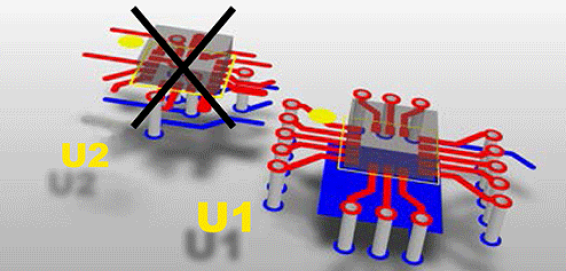
\includegraphics[width=0.5\textwidth]{img/IMU_recomendaciones_layout.png}
    \caption{Se muestran dos ejemplos de layout de una IMU. El layout U2 no sigue las recomendaciones mencionadas, mientras que U1 sí. La imagen se extrajo de \cite{IMUpcb_3}.}
    \label{fig:IMU_recomendaciones_layout}
\end{figure}

La imagen de la figura \ref{fig:IMU_recomendaciones_layout} resume algunas de estas recomendaciones. Lo que se observa es que las pistas del sensor son simétricas. A pesar de que algunos terminales de la IMU no se utilicen, se recomienda que igualmente sean incluidas en el routeo, solo para mantener la simetría. Durante el proceso de soldadura, el estaño presente en los distintos pads del componente generan una tensión que atrae el componente hacia este. En la figura \ref{fig:IMU_missalignment} se muestra un ejemplo de una IMU rotada respecto de su placa. Si el routeo no es simétrico, es posible que el sensor no quede centrado, lo que resultaría en un problema durante el uso de la computadora de vuelo.

\begin{figure}[H]
    \centering
    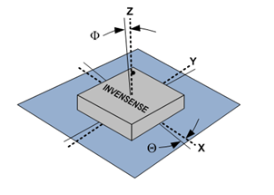
\includegraphics[width=0.4\textwidth]{img/IMU_missalignment.png}
    \caption{Se muestra un ejemplo donde la IMU se encuentra rotada respecto de la placa. En línea punteada los ejes de la terna solidaria al sensor y en línea continua la terna solidaria a la placa. La imagen se extrajo de \cite{IMUpcb_4}.}
    \label{fig:IMU_missalignment}
\end{figure}

%\subsubsection{Definición de las Características del PCB}

\subsubsection{Características del PCB}

Dada la gran cantidad de pistas que deben trazarse en toda la placa, se opta por un diseño de PCB de 4 capas. Esta elección simplifica el routeo, ya que se cuenta con una mayor cantidad de capas para pasar pistas, en relación a una configuración típica de 2 capas. En la figura \ref{fig:stackup} se muestra el \textit{stackup} utilizado para el PCB, donde se puede ver que se cuenta con 2 capas de señal, 1 capa de alimentación y 1 capa de retorno GND.

\begin{figure}[H]
    \centering
    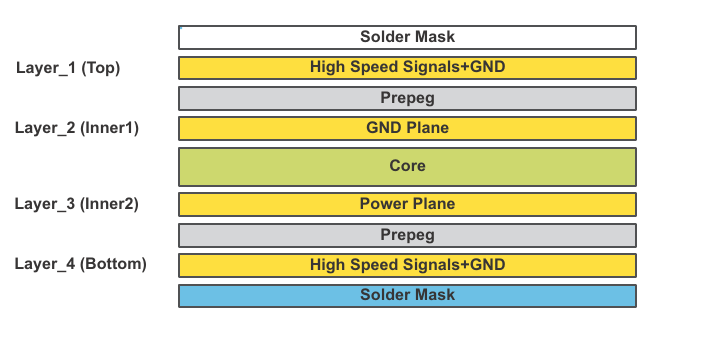
\includegraphics[width=0.7\textwidth]{img/stackup.png}
    \caption{Configuración de capas utilizada para el PCB. {\color{red} REEMPLAZAR ESTA IMAGEN POR UNA DIBUJADA POR MI. APROVECHAR Y AGREGAR LAS DIMENSIONES DEL ESPACIADO ENTRE CAPAS, EL ESPESOR DE COBRE Y LOS DIELÉCTRICOS.}}
    \label{fig:stackup}
\end{figure}

%\textbf{{\color{red} HABLAR DE LAS BONDADES DE PCB DE 4 CAPAS CON ESTA CONFIGURACIÓN (LIBRO OTT). MENCIONAR EL TEMA DE LAS PISTAS QUE REQUIEREN CIERTA IMPEDANCIA CARACTERÍSTICA}}

% Durante el desarrollo del PCB, se tuvieron en cuenta distintas cuestiones relacionadas a integridad de señal y a compatibilidad electromagnética. En muchos desarrollos de PCBs es común que se sigan una serie de lineamientos que se suelen llamar las ``buenas prácticas''. Muchas veces estas ofrecen soluciones de manera práctica a problemas ya conocidos, por ejemplo para asegurar la integridad de señales digitales.



% En este trabajo no se hizo una evaluación formal de estos aspectos en la computadora de vuelo, se siguieron los análisis planteados en el libro \textit{Electromagnetic Compatibility} de Henry Ott \cite{ott2011electromagnetic}.

La configuración de 4 capas tiene otras ventajas respeto del uso de 2. El circuito de la computadora de vuelo es prácticamente un circuito con señales digitales, por lo que debe darse un cuidado especial, minimizando la impedancia del retorno de corriente. En el caso de un PCB de 4 capas, al tener una capa entera dedicada al retorno, esta ofrecerá una muy baja impedancia para las corrientes de alta frecuencia. En la figura \ref{fig:ground_bounce} se muestra cómo el efecto de la inductancia presente en el retorno de señal, puede generar ruido a través de la conexión a GND en otros componentes. El ejemplo de la figura es con compuertas lógicas, pero aplica igualmente a cualquier circuito digital, por ejemplo a la comunicación entre el microcontrolador y alguno de los sensores.

%\textbf{{\color{red} AGREGAR UNA IMAGEN ILUSTRATIVA DE CÓMO LA IMPEDANCIA DEL RETORNO GENERA RUIDO EN GND. LA TENGO QUE DIBUJAR YO}}

\begin{figure}[H]
    \centering
    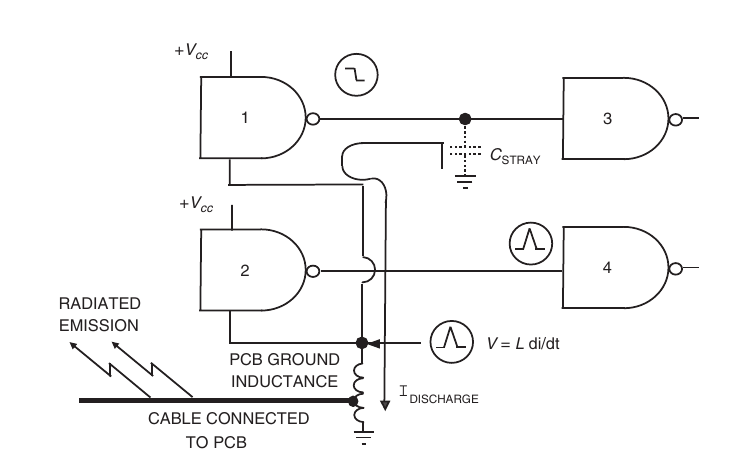
\includegraphics[width=0.7\textwidth]{img/ground_bounce.png}
    \caption{La compuerta lógica 2 mantiene su salida siempre en $0 \ V$, mientras que la compuerta lógica 1 conmuta su salida de estado alto a $0 \ V$. En este momento, se produce una descarga del capacitor $C_{STRAY}$ el cual representa capacidades que pueden ser por ejemplo de la pista que una su salida con la compuerta 3. En ese momento, la corriente circula por la inductancia del retorno, generando una caída de tensión que afecta a la compuerta 2 y a su salida. La imagen se extrajo de \cite[p.~381]{ott2011electromagnetic}.}
    \label{fig:ground_bounce}
\end{figure}

%minimizando el ruido que se propaga a otros componentes del circuito a través de la conexión a GND. 
En el caso de un PCB de 2 capas, es difícil reducir este efecto, ya que no se cuenta con el espacio suficiente. Otra de las ventajas es la disminución de las emisiones radiadas generadas por las caídas de potencial en la inductancia del retorno de señal \cite[p.~477]{ott2011electromagnetic}.

%\textbf{{\color{red} SE PODRÍA INCLUIR UNA IMAGEN ILUSTRATIVA DE CÓMO LA IMPEDANCIA DEL RETORNO GENERA RUIDO}}

%El uso de un PCB de 4 capas tiene muchas otras ventajas asociadas a aspectos de compatibilidad electromagnética, como la disminución de las emisiones radiadas generadas por las caídas de potencial en la inductancia del retorno de señal \cite[p.~477]{ott2011electromagnetic}.

%( Electromagnetic Compatibility de Henry Ott, capítulo 16.4.2.2. ).


%Al tratarse de un circuito con señales enteramente digitales, todas ellas presentarán componentes de altas frecuencias, ya sea para comunicación por ejemplo con la Micro SD, como también propias del funcionamiento del microcontrolador. Para altas frecuencias, las corrientes de retorno pueden generar diferencias de potencial producto del paso la corriente por las impedancias del retorno a GND. En la figura  se muestra un ejemplo para una señal digital donde se puede ver el efecto de la caída de tensión en la impedancia del retorno.


%En un PCB de 2 capas es difícil reducir este efecto, ya que no se cuenta con el espacio suficiente. En el caso de un PCB de 4 capas, al tener una capa entera dedicada al retorno, esta ofrecerá una muy baja impedancia en el retorno de las corrientes de alta frecuencia, por ende minimizando el ruido que se propaga a otros componentes del circuito, a través de su conexión a GND.


%Esto disminuye muchísimo las diferencias de potencial generadas producto del paso de estas corrientes de retorono por la impedancia de GND, con respecto a un PCB de solamente 2 capas. Estas diferencias de potencial se traducen en ruido que se propaga a otros componentes del circuito, a través de su conexión a GND.

%El hecho de disminuir las caidas de tensión en el plano de retorno trae consigo el efecto de disminuir las emisiones radiadas de modo común. Esto se debe a que las diferencias de potencial en el plano de retorno generan emisiones a través de los cables conectados al PCB ( Electromagnetic Compatibility de Henry Ott, capítulo 16.4.2.2. ).

%La ventaja principal es el hecho de contar con planos enteros de alimentación y de retorno. Minimizan las inductancias en el camino de la señal de corriente entregada a los componentes digitales, principalmente el microcontrolador. Esto minimiza el ruido producto de las conmutaciones.

%El uso de un plano de GND permite trabajar con pistas tipo \textit{microstrip} de impedancia característica conocida. Para algunas de las señales de la placa, es necesario que el camino de señal tenga cierta impedancia característica, como es el caso de USB y Micro SD.


%Otra de las ventajas es que pueden diseñarse pistas de impedancia controlada de pequeñas dimensiones. Esto se necesario para varias pistas, por ejemplo microSD y USB.

La selección del espaciado entre placas y el espesor de cobre se vieron afectadas por las posibilidades ofrecidas por el fabricante \textit{PCBWay}. Se optó por la opción más económica, correspondiente a las dimensiones de la figura \ref{fig:stackup}.

%\textbf{{\color{red} CAPACITORES DE DESACOPLE EN TODOS LOS COMPONENTES CON MONTAJE CON INDUCTANCIA MÍNIMA.}}

Otra de las técnicas utilizadas para reducir el ruido producto de las corrientes de alta frecuencia en la placa es el agregado de capacitores de desacople, principalmente en el microcontrolador. Estos ofrecen un camino de baja impedancia descargándose y entregando corrientes de alta frecuencia.

%\textbf{{\color{red} MENCIONAR QUE LA PLACA TIENE 3,3V Y 5V Y QUE SE OPTÓ POR UNA PISTA EN LA CAPA TOP, A DIFERENCIA DE UN PLANO.}}

Algunos de los conectores de la computadora de vuelo tienen salidas con tensiones de $5 \ V$ utilizados para alimentar módulos y sensores, como es el caso del receptor GPS. Esta tensión de $5 \ V$ se obtiene directamente desde la tensión de entrada del conector de alimentación de la computadora de vuelo. Para ello, se trazó una pista en la misma cara top, con un ancho mayor al resto de las demás. Esta se muestra en la figura \ref{fig:pista_5V}. Podría haberse incluido un plano con esta tensión en la misma capa que el plano de $3.3 \ V$. Sin embargo, esto hubiera generado que el plano de $3.3 \ V$ se viera afectado, haciendo que este se viera partido, lo que incrementaría la impedancia vista por las corrientes sobre este.

\begin{figure}[H]
    \centering
    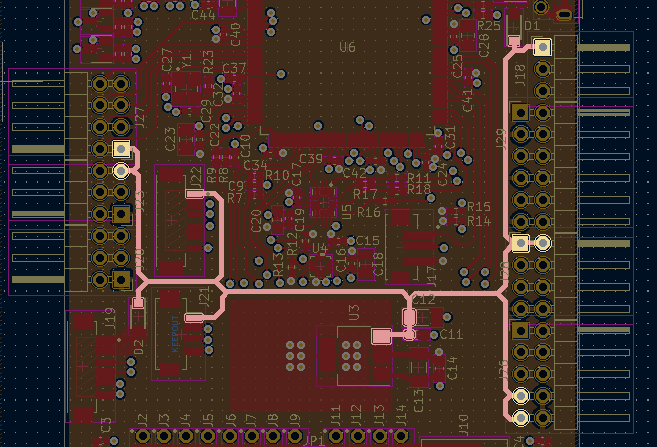
\includegraphics[width=\textwidth]{img/pista_5V.png}
    \caption{Se muestra una captura del software KiCad, utilizado para el desarrollo de la placa de la computadora de vuelo. Se resalta la pista de $5 \ V$ en la capa top. A su vez se puede ver la zona naranja la cual corresponde a la capa 3 y que contiene en su totalidad al plano de $3.3 \ V$. El plano de GND se ubica en la capa 2.}
    \label{fig:pista_5V}
\end{figure}



%Si bien la tensión de alimentación de la computadora de vuelo son $3.3 \ V$, algunos de sus conectores entregan tensiones de $5 \ V$ necesarias para aliemntar ciertos módulos y sensores externos, por ejemplo el sensor GPS. Esta tensión se obtiene directamente desde la tensión de entrada del conector de alimentación de la computadora de vuelo.


%La tensión de alimentación de la computadora de vuelo son $5 \ V$, la cual se utiliza para alimentar el regulador lineal y generar los $3.3 \ V$. 







Al tener varias capas, el routeo de las pistas traerá una gran cantidad de vías en la placa. Existen distintos tipos de vías que ofrece el fabricante, estas se muestran en la figura \ref{fig:vias_PCB}. Se prefiere evitar el uso de otro tipo de vía que no sea una vía pasante, debido a que de otra forma, incrementaría mucho el costo de fabricación de la placa.

\begin{figure}[H]
    \centering
    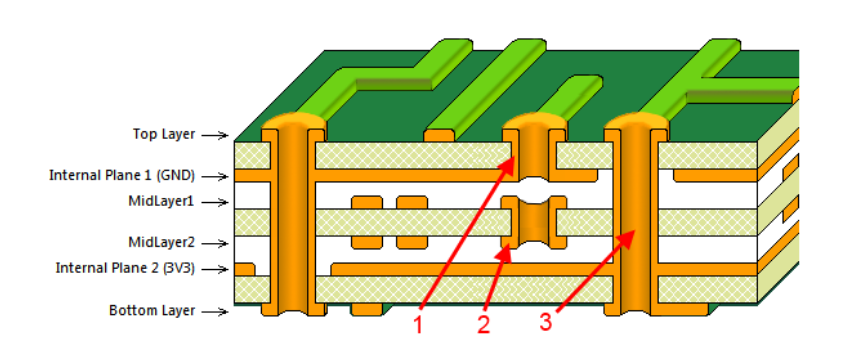
\includegraphics[width=0.8\textwidth]{img/vias_PCB.png}
    \caption{La vía 1 corresponde a una vía ciega (\textit{blind via}), la 2 corresponde a una \textit{buried via} y la 3 a una vía pasante. El uso de vías ciegas ayuda a reducir el espacio ocupado por un circuito en un PCB, ya que permite colocar componentes por encima de estas. La desventaja que traen es que su uso incrementa mucho el costo de fabricación de la placa, ya que el proceso de manufactura de las mismas es más complejo que el de las vías pasantes.}
    \label{fig:vias_PCB}
\end{figure}


%\textbf{{\color{red} COMPLETAR}}

\subsubsection{Comunicación con el Slot para Tarjeta Micro SD}

% Length matching e impedancia característica. Mencionar todo lo que tengo de la especificación de microSD. Tengo muchísimo de esto.

\textbf{{\color{red} MENCIONAR EL TEMA DE LAS PISTAS QUE REQUIEREN CIERTA IMPEDANCIA CARACTERÍSTICA Y CÓMO ES QUE EL STACK DEL PCB AYUDA A TENER DIMENSIONES PEQUEÑAS}}

\textbf{{\color{red} COMPLETAR}}

\subsubsection{Comunicación USB}

% Impedancia característica de la pista diferencial, de la especificación.

\textbf{{\color{red} COMPLETAR}}

\subsubsection{Layout del Regulador Lineal}

\textbf{{\color{red} COMPLETAR}}

\subsection{Funcionalidades y Diagrama en Bloques}

% Acá lo que hago es mencionar cuáles son las necesidades con las que tengo que cumplir con la placa y después muestro un diagrama en bloques. Todavía no doy ningún circuito, es todo a nivel de sistema.

% Procesa datos de los sensores
% Actúa sobre los motores
% Administra interfaces de comunicación externa (CAN, UART, I2C, SPI, USB, SWD)
% Calcular la ley de control
% Almacenamiento de datos recolectados por la computadora de vuelo, ya sea del vuelo o de la aplicación.
% LEDs indicadores de propósito general.
% Pulsadores para debugging y pruebas de propósito general.

La computadora de vuelo tiene la tarea esencial de adquirir las mediciones de los sensores, procesar dichos datos, y realizar el control de los diversos aspectos del vehículo, fundamentalmente de los motores. Las funcionalidades de la computadora de vuelo son las siguientes:

\begin{enumerate}
    \item Adquirir datos de sensores.
    \item Cálculo de la estimación de la pose y de la ley de control.
    \item Actuación sobre los motores.
    \item \textbf{{\color{red} FALTA ALGUNA FUNCIONALIDAD DE TOLERANCIA A FALLAS}}
    \item Control de LEDs indicadores de propósito general.
    \item Comunicación a través de distintas interfaces, con módulos y sensores externos a la placa.
    \item Loggeo de datos.
\end{enumerate}

\begin{figure}[H]
    \centering
    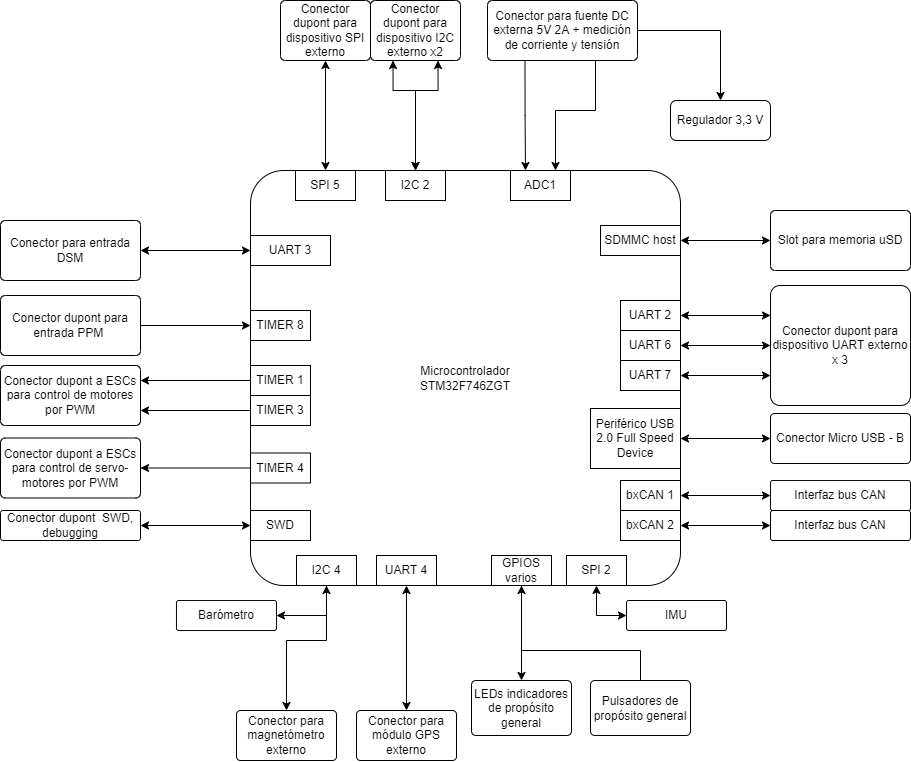
\includegraphics[width=\textwidth]{img/diagrama_en_bloques_computadora_de_vuelo.png}
    \caption{Diagrama en bloques de la computadora de vuelo.}
    \label{fig:diagrama_en_bloques_computadora_de_vuelo}
\end{figure}

\textbf{{\color{red} AGREGAR UNA FOTO DEL PCB, CON FLECHAS INDICANDO DÓNDE ESTÁ CADA COSA}}

\textbf{{\color{red} COMPLETAR}}